%%==============================================================
%% Modelo de TCC para o curso de Sistemas de Informação
%% da Universidade Federal de Viçosa - Campus de Rio Paranaíba
%% Autor: Rodrigo Smarzaro (smarzaro@ufv.br)
%% Última versão Março/2014
%% Arquivo em formato UTF-8
%% Compilar com pdftex
% %Precisa do arquivo UFV.sty
%%==============================================================

\documentclass[
	% -- opções da classe memoir --
	12pt,				    % tamanho da fonte
	openright,			    % capítulos começam em pág ímpar (insere página vazia caso preciso)
	oneside,			    % para impressão só no anverso. Oposto a twoside
	a4paper,			    % tamanho do papel.
    % -- opções do pacote abntex2 --
    % chapter=TITLE,         % Títulos em maiúsculas
    sumario=tradicional,    % Sumário padrão memoir (mais bonito "imo")
    % -- opções do pacote babel --
	english,			    % idioma adicional para hifenização
	brazil,				    % o último idioma é o principal do documento
	]{abntex2}              % Personaliza a capa. Precisa do arquivo ufv.cls para funcionar.



% Pacotes fundamentais
\usepackage{abntex2-UFV}        % Personalização para a Universidade Federal de Viçosa
\usepackage{lmodern}			% Usa a fonte Latin Modern			
\usepackage[T1]{fontenc}		% Selecao de codigos de fonte de saída
\usepackage[utf8]{inputenc}		% Codificacao do documento (conversão automática dos acentos)
\usepackage{indentfirst}		% Indenta o primeiro parágrafo de cada seção.
\usepackage{graphicx}			% Inclusão de gráficos
\usepackage{booktabs}           % \toprule, \midrule e \bottomrule para tabelas
% Sistema autor-data com títulos nas referências em negrito
\usepackage[alf,abnt-emphasize=bf]{abntex2cite}	
\usepackage{pdfpages}



% ---
% CONFIGURAÇÕES DE PACOTES
% ---

% Informações de dados para CAPA e FOLHA DE ROSTO
\titulo{SheSafe – Aplicativo de pedido de ajuda para mulheres em situação de risco}
\autor{Lucas de Oliveira Macêdo}
\local{São Carlos}
\data{2025}
\orientador{Silvana Maria Affonso de Lara}    % redefinido no abntex2-UFV para aceitar Instituição (default = UFV-CRP)
%\coorientador{Nome do Coorientador}
\instituicao{Instituto Federal de São Paulo}

\campus{\emph{Campus} de São Carlos}      % pacote abntex2-UFV
\curso{Pós-Graduação \emph{Lato Sensu} em
Desenvolvimento de Sistemas para Dispositivos Móveis}               % pacote abntex2-UFV
\membrobancaA{Membro da Banca A}             % pacote abntex2-UFV default = UFV-CRP
\membrobancaB[UFMG]{Membro da Banca B}       % pacote abntex2-UFV default = UFV-CRP
\databanca{\today}                           % pacote abntex2-UFV

% O preambulo deve conter o tipo do trabalho, o objetivo,
% o nome da instituição e a área de concentração
\preambulo{Trabalho de conclusão apresentado ao Instituto Federal de São Paulo para obtenção do título de Especialista em Desenvolvimento para Dispositivos Móveis. }
% ---

% ---
% Configurações de aparência do PDF final

% informações para o arquivo pdf de saída
% Interessante alterar a cor dos links para preto(black)
% para imprimir
\makeatletter
\hypersetup{
        % metadados
		pdftitle={\@title},
		pdfauthor={\@author},
    	pdfsubject={\imprimirpreambulo},
	    pdfcreator={LaTeX with abnTeX2},
		colorlinks=true,   % false: links em frame; true: links coloridos
    	linkcolor=black,    % cor dos links no documento
    	citecolor=blue,    % cor dos links para a bibliografia
    	filecolor=magenta, % cor dos links para arquivos
		urlcolor=blue,     % cor dos links para sites
		bookmarksdepth=4   % profundidade do sumário do PDF
}
\makeatother
% ---

\begin{document}
% Retira espaço extra obsoleto entre as frases.
\frenchspacing

% ----------------------------------------------------------
% ELEMENTOS PRÉ-TEXTUAIS
% ----------------------------------------------------------
\pretextual

% Capa
\imprimircapa

% Folha de rosto
\imprimirfolhaderosto
% ---

% Inserir folha de aprovação
%\imprimirfolhadeaprovacao

% Dedicatória
%\begin{dedicatoria}
%   \vspace*{\fill}
%   \centering
%   \noindent
%   \textit{Texto qualquer da dedicatória}
%   \vspace*{\fill}
%\end{dedicatoria}
% ---

% Agradecimentos
%\begin{agradecimentos}

%\end{agradecimentos}
 ---

% Epígrafe
%\begin{epigrafe}
%    \vspace*{\fill}
%	\begin{flushright}
%		\textit{``Word? nunca mais.''\\
%		(Qualquer usuário de \LaTeX)}
%	\end{flushright}
%\end{epigrafe}
% ---

% RESUMOS

% resumo em português
\begin{resumo}
 \noindent
%Insira o resumo aqui
A violência contra a mulher constitui um problema de saúde pública global de proporções epidêmicas, afetando aproximadamente 770 milhões de mulheres anualmente em relacionamentos com parceiros ou ex-parceiros. A pandemia da COVID-19 agravou significativamente este cenário, uma vez que o isolamento social, principal medida de contenção adotada, criou condições propícias para o fortalecimento dos elementos de violência doméstica, mantendo as vítimas por períodos prolongados sob controle direto de seus agressores. Consequentemente, observou-se um aumento expressivo dos casos de violência contra a mulher durante o período pandêmico, intensificando uma tendência de crescimento já identificada anteriormente.

 \vspace{\onelineskip}

 \noindent
 \textbf{Palavras-chaves}: Violência contra a mulher. Aplicação mobile. Geolocalização. Pedido de socorro. Proteção da mulher. Violência doméstica.
\end{resumo}

% resumo em inglês
\begin{resumo}[Abstract]
 \begin{otherlanguage*}{english}
   \noindent
%   % Insira o abstract aqui
Violence against women is a global public health problem of epidemic proportions, affecting approximately 770 million women annually in relationships with current or former partners. The COVID-19 pandemic has significantly worsened this situation, as social isolation, the primary containment measure imposed, created conditions conducive to the intensification of domestic violence, keeping victims under the direct control of their aggressors for prolonged periods. Consequently, there was a significant increase in cases of violence against women during the pandemic, intensifying a previously observed upward trend.

   \vspace{\onelineskip}

   \noindent
   \textbf{Key-words}: Violence against women. Mobile application. Geolocation. Call for help. Women's protection. Domestic violence.
 \end{otherlanguage*}
\end{resumo}

% inserir lista de ilustrações
\pdfbookmark[0]{\listfigurename}{lof}
\listoffigures*
\cleardoublepage
% ---

% inserir lista de tabelas
% \pdfbookmark[0]{\listtablename}{lot}
% \listoftables*
% \cleardoublepage
% ---


% Lista de siglas e abreviaturas (opcional)
% sintaxe: \item [sigla] Descrição da sigla

%\begin{siglas}
%\item[ABNT] Absurdas Normas Técnicas
%\item[UFV] Universidade Federal de Viçosa
%\item[CRP] \emph{Campus} de Rio Paranaíba
%\end{siglas}

% Lista de símbolos (opcional)
% sintaxe: \item [simbolo] Descrição do símbolo

%\begin{simbolos}
%\item[$\infty$ ] Infinito
%\end{simbolos}


% inserir o sumario
\pdfbookmark[0]{\contentsname}{toc}
\tableofcontents*
\cleardoublepage
% ---



% ----------------------------------------------------------
% ELEMENTOS TEXTUAIS
% ----------------------------------------------------------
\textual


%Modifique a estrutura dos capítulos e seções de acordo com a necessidade do seu trabalho
\chapter{Introdução}\label{sec:introducao}
O isolamento social durante o período de pandemia acabou se tornado um fator primordial no aumento dos conflitos familiares, isso obrigou a mulheres, que convivem com seus agressores, a permanecerem por um período mais longo junto a eles. Embora haja visto um aumento no número de casos de violência contra a mulher, constata-se, segundo dados da Cartilha de Violência contra a mulher de maio de 2020, que o número de denúncias diminuiu. Tal fato se dá pela proximidade da vítima ao agressor, pelo sequestro de subjetividade, pela precariedade do serviço público e pelo medo de sair do isolamento, dentre outros fatores.

\section{Escopo do Projeto}
O escopo do projeto tem como base oferecer uma aplicação simples, intuitiva e de fácil acesso ao nosso público-alvo para que estes sejam capazes de enviar um pedido de ajuda, para pessoas de sua confiança, em momentos que estiverem passando por uma situação de risco, agressão ou até mesmo violência. Estes pedidos de ajuda informarão a essas pessoas de confiança, na aplicação denominadas de “contatos seguros”, a localização atual do usuário juntamente com uma mensagem predefinida por ele.

\section{Público-alvo}
SheSafe tem como público-alvo pessoas do sexo feminino que desejam ter uma forma de comunicar a pessoas de sua confiança algum potencial risco; seja ele violência, agressão, insegurança na rua, perseguição por algum individuo ou outro risco qualquer, que estiver passando em tempo real

\section{Mapa de empatia inicial}
\begin{figure}[htbp]
  \begin{center}
  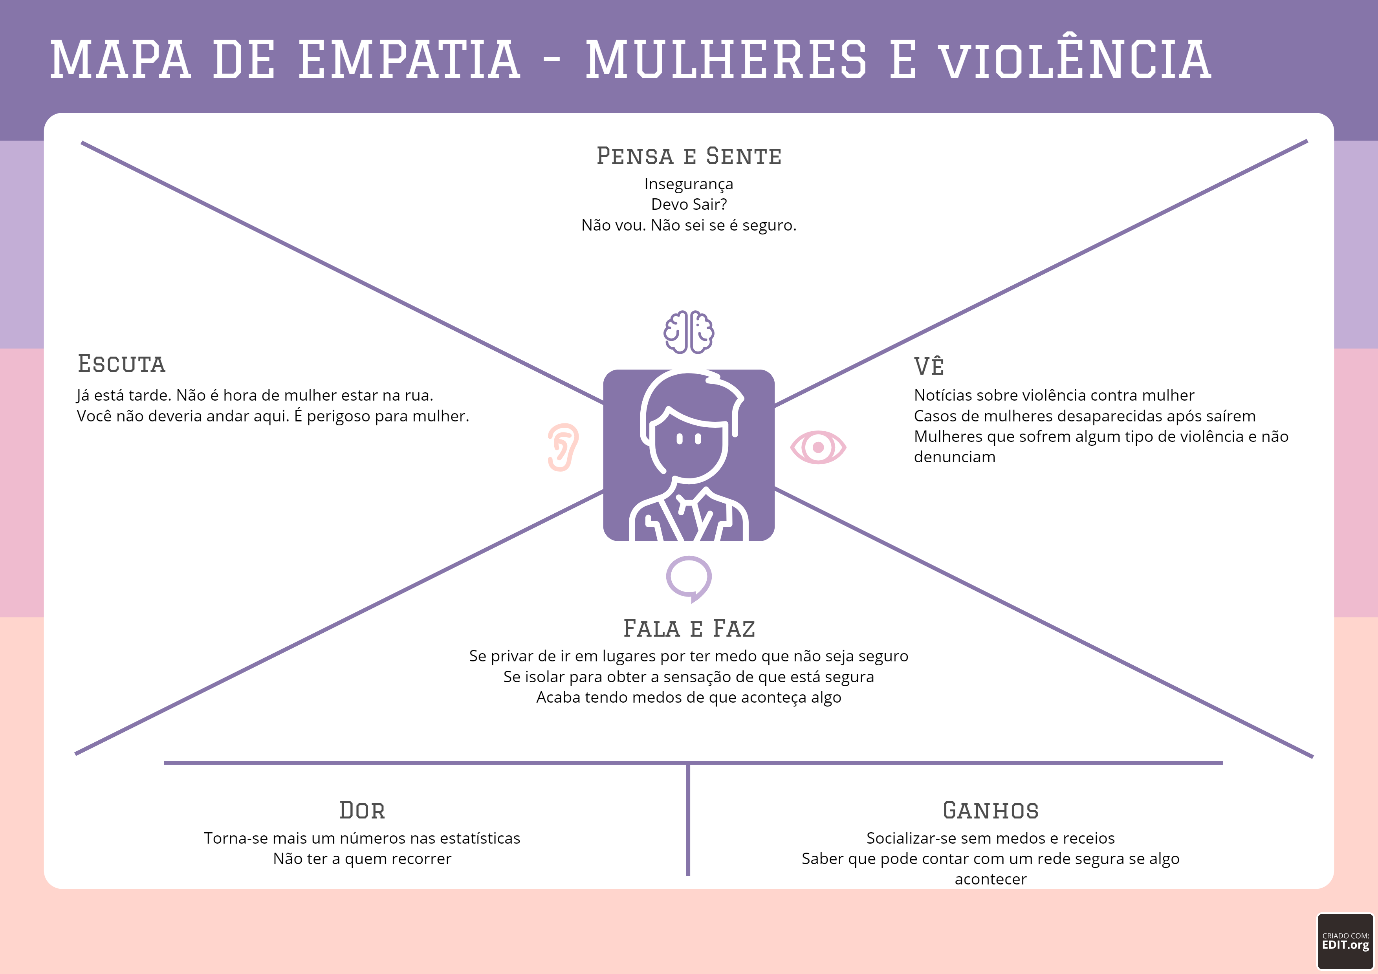
\includegraphics[width=.9\linewidth]{images/mapa-empatia-inicial.png}\\
  \end{center}
  \caption[Mapa de empatia inicial]{Mapa de empatia inicial sobre sentimento das mulheres sobre violência}
  \label{fig:mapa-empatia-inicial}
  \legend{Fonte: Próprio Autor}
\end{figure}

\section{Ambiente de uso}
O SheSafe poderá ser utilizado em qualquer ambiente desde que se tenha um plano de internet ativo para que os pedidos de ajuda possam ser enviados corretamente para a lista de contatos seguros. Uma outra restrição quanto ao uso é que os usuários devem possuir um smartphone com sistema operacional Android ou iOS para que possam instalar o aplicativo.

\section{Restrições de Uso/Circunstâncias}
Não há restrições quanto ao uso do SheSafe. Caso o usuário sinta-se em situação de risco ele poderá acionar o aplicativo e enviar seu pedido de ajuda, desde que já tenha cadastrado sua lista de contatos seguros.

\section{Diferencial}
Dado que muito dos casos de agressão acontecem com mulheres em situação de risco e muitas das vezes elas são privadas de acesso a formas de comunicação mais tecnológicas, o intuito é ter uma aplicação onde as mulheres possam reportar crimes de forma simples, prática e disponível para todos os públicos. O principal diferencial está em não restringir o acesso a aplicação para nosso público-alvo e ter a opção de envio da localização no momento do acontecimento.

\section{Funcionalidades mínimas para garantir a relevância do aplicativo}
As funcionalidades mínimas elencadas para que o projeto tenha relevância são:
\begin{alineas}
  \item Login: Para criação de usuário
  \item Pedido de socorro: Botão para acionar pedido de socorro
  \item Lista Segura: Gerenciamento de contatos seguros
  \item Perfil: Página para alteração da mensagem de socorro

\end{alineas}


\chapter{Referencial Teórico}\label{sec:RefTeorico}
\section{Sistema operacional Android}

O Android constitui-se como um sistema operacional fundamentado no núcleo Linux, atualmente sob desenvolvimento e manutenção da empresa Google Inc. \cite{google2023}. Este sistema operacional caracteriza-se por uma arquitetura de interface baseada em manipulação direta, sendo especificamente projetado para atender às demandas de dispositivos móveis equipados com tecnologia de tela sensível ao toque, incluindo smartphones e tablets \cite{burnette2021}.

A versatilidade da plataforma Android estende-se para além dos dispositivos móveis convencionais, abrangendo uma ampla gama de equipamentos tecnológicos. Neste contexto, destacam-se as adaptações específicas como o Android TV para televisores inteligentes, o Android Auto para sistemas automotivos e o Android Wear para dispositivos vestíveis, particularmente relógios inteligentes \cite{ableson2022}. O sistema utiliza recursos de interface intuitiva, empregando a tecnologia de tela sensível ao toque para permitir que os usuários manipulem objetos virtuais através de gestos diretos, complementada por um teclado virtual integrado.

Embora o Android tenha sido concebido primordialmente para dispositivos com interface touchscreen, sua aplicabilidade transcende esta categoria, sendo implementado em consoles de videogames, câmeras digitais, computadores pessoais e diversos outros equipamentos eletrônicos \cite{murphy2023}. Esta flexibilidade arquitetural demonstra a robustez e adaptabilidade da plataforma para diferentes contextos de uso.

\subsection{Posicionamento no Mercado Global}

Dados estatísticos revelam a significativa penetração do sistema Android no mercado mundial de sistemas operacionais. Segundo levantamento conduzido pela StatCounter Global Stats \cite{statcounter2017}, empresa especializada em pesquisas e análises estatísticas de mercado tecnológico, em março de 2017, os usuários do Android representavam 37,93\% da atividade global em redes, superando ligeiramente o sistema Windows, que registrou 37,91\% no mesmo período. Estes números consolidaram o Android como o sistema operacional mais utilizado mundialmente, marcando um ponto de inflexão significativo no panorama tecnológico global.

No âmbito do desenvolvimento de aplicações móveis, pesquisa conduzida entre programadores durante o período de abril a maio de 2013 evidenciou que 71\% dos desenvolvedores direcionavam seus esforços para a plataforma Android \cite{developereconomics2013}. Esta preferência dos desenvolvedores reflete tanto a popularidade do sistema quanto as oportunidades de mercado que a plataforma oferece.

\subsection{Características de Licenciamento e Código Aberto}

Um aspecto fundamental que distingue o Android de outros sistemas operacionais móveis refere-se ao seu modelo de licenciamento. O sistema operacional distribuído pela Google opera sob licença de código aberto (open source), fundamentada na Apache License 2.0 \cite{opensource2023}, garantindo aos desenvolvedores e programadores os direitos fundamentais de estudar, modificar e distribuir o software de forma gratuita.

Esta característica de código aberto proporciona liberdade significativa para qualquer indivíduo ou organização utilizar o sistema para qualquer finalidade, sem restrições de uso comercial ou não comercial. No entanto, é importante destacar que, embora o núcleo do sistema Android seja distribuído como software livre, a maioria dos dispositivos comerciais são lançados com uma combinação híbrida de software livre e software proprietário, incluindo aplicativos e serviços específicos do fabricante ou do Google \cite{lee2022}.

\section{Android Studio}
\subsection{Caracterização e Fundamentação Técnica}

O Android Studio constitui-se como o ambiente de desenvolvimento integrado (IDE - Integrated Development Environment) oficial designado pela Google para o desenvolvimento de aplicações móveis destinadas à plataforma Android \cite{google2023androidstudio}. Esta ferramenta de desenvolvimento fundamenta-se na arquitetura do IntelliJ IDEA, uma das principais plataformas de desenvolvimento Java desenvolvida pela JetBrains, incorporando suas funcionalidades centrais de edição de código e ferramentas avançadas de desenvolvimento \cite{jetbrains2023intellij}.

A escolha do IntelliJ IDEA como base arquitetural para o Android Studio justifica-se pela robustez e maturidade desta plataforma no ecossistema de desenvolvimento Java, linguagem predominante no desenvolvimento Android tradicional. Esta decisão estratégica permitiu à Google herdar um conjunto consolidado de funcionalidades de desenvolvimento, enquanto adiciona camadas especializadas voltadas especificamente para as particularidades do desenvolvimento móvel Android \cite{meier2023android}.

\subsection{Funcionalidades e Recursos Especializados}

O Android Studio incorpora um conjunto abrangente de funcionalidades específicas para otimizar o processo de desenvolvimento de aplicações Android, transcendendo as capacidades básicas de edição de código. Entre os recursos mais significativos para a produtividade do desenvolvedor, destacam-se elementos fundamentais que caracterizam a modernidade e eficiência da plataforma.

O sistema de compilação integrado baseia-se na ferramenta Gradle, um sistema de automação de build de código aberto que oferece flexibilidade superior aos sistemas tradicionais baseados em XML, como o Apache Maven \cite{gradle2023build}. Esta integração proporciona gerenciamento automatizado de dependências, compilação incremental e configuração modular de projetos, elementos essenciais para o desenvolvimento escalável de aplicações complexas.

A plataforma incorpora um emulador Android de alta performance, desenvolvido com tecnologias de virtualização otimizadas que permitem a simulação eficiente de diversos dispositivos Android sem a necessidade de hardware físico \cite{google2023emulator}. Este recurso é fundamental para testes de compatibilidade e validação de funcionalidades em diferentes configurações de hardware e versões do sistema operacional.

O ambiente oferece suporte unificado para desenvolvimento direcionado a múltiplas categorias de dispositivos Android, incluindo smartphones, tablets, dispositivos vestíveis (wearables), sistemas automotivos e televisores inteligentes. Esta abordagem unificada simplifica significativamente o processo de desenvolvimento para ecossistemas heterogêneos de dispositivos \cite{ableson2023multiplatform}.

\subsection{Recursos de Desenvolvimento Ágil e Qualidade de Código}

O Android Studio implementa funcionalidades avançadas voltadas para metodologias de desenvolvimento ágil e manutenção da qualidade de código. O recurso Instant Run representa uma inovação significativa no ciclo de desenvolvimento, permitindo a aplicação de alterações de código diretamente em aplicações em execução, eliminando a necessidade de recompilação completa do arquivo APK (Android Package) \cite{google2022instantrun}. Esta funcionalidade reduz substancialmente o tempo de iteração durante o processo de desenvolvimento e depuração.

A integração nativa com sistemas de controle de versão, particularmente o GitHub, facilita a colaboração em equipes de desenvolvimento e o gerenciamento de código fonte \cite{github2023integration}. Adicionalmente, a plataforma disponibiliza modelos de código pré-configurados (code templates) que aceleram o desenvolvimento de funcionalidades comuns e promovem a padronização de práticas de codificação.

O ambiente incorpora um conjunto robusto de ferramentas e frameworks para implementação de testes automatizados, abrangendo testes unitários, testes de integração e testes de interface do usuário \cite{junit2023android}. Estas funcionalidades são complementadas por ferramentas especializadas de análise estática de código, capazes de identificar potenciais problemas relacionados a performance, usabilidade, compatibilidade entre versões do Android e outras questões críticas para a qualidade da aplicação final \cite{android2023lint}.

\iffalse
\begin{figure}[htbp]
  \begin{center}
  
\includegraphics[width=.5\linewidth]{images/logo-ifsp.png}\\
  \end{center}
  \caption[Exemplo de Figura]{Exemplo de inserção de figura no \LaTeX. A legenda deve vir abaixo da figura. Pode usar o comando \texttt{\textbackslash legend} ou \texttt{\textbackslash fonte} para inserir a fonte da figura. Observe que na lista de ilustrações foi utilizado o nome curto fornecido como parâmetro do caption da figura (veja o arquivo fonte .tex) ao invés dessa legenda estupidamente extensa feita de forma proposital}
  \label{fig:logo}
  \legend{Fonte: Próprio Autor}
\end{figure}
\fi
\section{Firebase}
\subsection{Caracterização e Contextualização Histórica}

O Firebase constitui-se como uma plataforma abrangente de desenvolvimento para aplicações móveis e web, tendo sido incorporada ao portfólio de soluções da Google Inc. em outubro de 2014 através de processo de aquisição estratégica \cite{google2014firebase}. Originalmente fundada em 2011 por James Tamplin e Andrew Lee, a plataforma Firebase foi concebida com o propósito de fornecer uma infraestrutura de backend-as-a-service (BaaS) completa e de alta usabilidade, direcionada especificamente para simplificar o processo de desenvolvimento e implementação de aplicações digitais \cite{tamplin2021firebase}.

A filosofia de desenvolvimento da plataforma fundamenta-se na disponibilização de um ecossistema integrado de serviços diversos, que abrangem desde funcionalidades básicas de armazenamento de dados até recursos avançados de análise comportamental e engajamento de usuários \cite{firebase2023docs}. Esta abordagem holística visa reduzir a complexidade técnica tradicionalmente associada ao desenvolvimento de backends customizados, permitindo que desenvolvedores concentrem seus esforços na criação de interfaces e experiências de usuário diferenciadas.

\subsection{Interface de Gerenciamento e Implementação}

A operacionalização da plataforma Firebase é mediada por um console web especializado, denominado Firebase Console, que representa a interface principal de gerenciamento e configuração de projetos \cite{google2023console}. Este ambiente de desenvolvimento integrado foi projetado seguindo princípios de experiência do usuário (UX) orientados à simplicidade e intuitividade, proporcionando aos desenvolvedores um fluxo de trabalho otimizado para implementação de recursos.

O processo de utilização inicia-se com a criação de um projeto no console, seguido pela seleção e configuração dos serviços desejados a partir de um catálogo extenso de funcionalidades disponíveis. Cada serviço oferecido pela plataforma é acompanhado de documentação técnica detalhada, incluindo guias de implementação passo-a-passo, exemplos de código e melhores práticas de desenvolvimento \cite{firebase2023implementation}.

\subsection{Modelo de Comercialização e Estrutura Tarifária}

O Firebase opera sob um modelo de negócios freemium, caracterizado pela disponibilização gratuita de funcionalidades básicas combinada com planos pagos para recursos avançados e maior capacidade de processamento \cite{google2023pricing}. Esta estrutura tarifária escalonável permite que desenvolvedores individuais e pequenas equipes iniciem projetos sem investimento inicial, enquanto organizações com demandas mais robustas podem optar por planos comerciais adequados às suas necessidades específicas.

A estratégia de precificação adotada segue uma lógica de pay-as-you-scale, onde os custos são proporcionais ao volume de utilização dos recursos, incluindo métricas como número de usuários ativos, volume de dados armazenados e quantidade de operações de leitura/escrita realizadas \cite{moroney2022firebase}. Esta abordagem visa garantir a viabilidade econômica tanto para projetos em fase inicial quanto para aplicações consolidadas com grande base de usuários.

\subsection{Firebase Authentication}

\subsubsection{Caracterização do Serviço e Arquitetura Funcional}

O Firebase Authentication constitui-se como um serviço especializado de autenticação e autorização de usuários, integrado ao ecossistema da plataforma Firebase, oferecendo uma solução abrangente de gerenciamento de identidade digital para aplicações móveis e web \cite{google2023firebaseauth}. Este serviço fundamenta-se em uma arquitetura de backend-as-a-service (BaaS) que disponibiliza infraestrutura completa de autenticação, eliminando a necessidade de desenvolvimento e manutenção de sistemas proprietários de gerenciamento de credenciais por parte dos desenvolvedores.

A arquitetura do Firebase Authentication baseia-se na provisão de serviços de backend robustos, complementados por kits de desenvolvimento de software (SDKs) otimizados e bibliotecas de interface de usuário pré-desenvolvidas \cite{firebase2023sdk}. Esta abordagem integrada visa simplificar significativamente o processo de implementação de funcionalidades de autenticação, permitindo que desenvolvedores foquem na lógica de negócio específica de suas aplicações, enquanto delegam a complexidade técnica da autenticação para a infraestrutura especializada do Firebase.

\subsubsection{Modalidades de Autenticação e Provedores de Identidade}

O sistema oferece suporte abrangente a múltiplas modalidades de autenticação, atendendo às diversas preferências e contextos de uso dos usuários finais. A plataforma implementa autenticação tradicional baseada em credenciais de senha, permitindo que usuários criem contas através de endereços de email e senhas personalizadas \cite{stallings2023cryptography}. Adicionalmente, o serviço incorpora funcionalidades de autenticação por meio de números de telefone, utilizando protocolos de verificação por SMS para validação de identidade.

Uma característica distintiva do Firebase Authentication reside em sua capacidade de integração com provedores de identidade federados, implementando o conceito de Single Sign-On (SSO) através de plataformas estabelecidas no mercado \cite{jones2022federated}. Entre os provedores suportados, destacam-se o Google, Facebook, Twitter, GitHub, Apple, Microsoft, Yahoo, além de suporte para provedores customizados através de protocolos padronizados. Esta diversidade de opções de autenticação visa atender às preferências individuais dos usuários e reduzir barreiras de entrada nas aplicações.

\subsubsection{Integração Sistêmica e Conformidade com Padrões da Indústria}

O Firebase Authentication foi projetado com foco na integração estreita com outros componentes do ecossistema Firebase, incluindo Firebase Firestore, Firebase Realtime Database, Firebase Cloud Functions e Firebase Analytics \cite{firebase2023ecosystem}. Esta integração sistêmica permite a implementação de regras de segurança baseadas em identidade de usuário, controle de acesso granular a recursos e personalização de experiências com base no perfil de autenticação.

A arquitetura do serviço fundamenta-se na aderência rigorosa a padrões industriais reconhecidos para autenticação e autorização, particularmente os protocolos OAuth 2.0 e OpenID Connect \cite{hardt2012oauth}. O OAuth 2.0 constitui-se como o padrão de facto para autorização de aplicações web e móveis, proporcionando mecanismos seguros para concessão de acesso limitado a recursos sem exposição de credenciais. Complementarmente, o OpenID Connect representa uma camada de identidade construída sobre o OAuth 2.0, fornecendo informações de identidade de usuário de forma padronizada \cite{sakimura2014openid}.

Esta conformidade com padrões estabelecidos facilita significativamente a integração do Firebase Authentication com sistemas de backend existentes, APIs de terceiros e infraestruturas corporativas, garantindo interoperabilidade e reduzindo a complexidade de implementação em arquiteturas híbridas ou migrações graduais de sistemas legados.


\subsection{Firebase Firestore}
\subsubsection{Caracterização e Arquitetura do Sistema}

O Firebase Firestore constitui-se como um banco de dados NoSQL (Not Only SQL) orientado a documentos, desenvolvido e mantido pela Google como componente central do ecossistema Firebase \cite{google2023firestore}. Esta solução de armazenamento fundamenta-se em uma arquitetura distribuída e escalável, projetada especificamente para atender às demandas de aplicações móveis e web modernas que requerem sincronização de dados em tempo real entre múltiplos clientes e dispositivos \cite{chang2008bigtable}.

A arquitetura do Firestore baseia-se no modelo de dados orientado a documentos, onde as informações são organizadas em estruturas hierárquicas compostas por coleções e documentos \cite{mongodb2023nosql}. Cada documento representa uma unidade de dados estruturada em formato JSON, contendo pares chave-valor que podem incluir tipos primitivos, arrays, objetos aninhados e referências a outros documentos. Esta flexibilidade estrutural permite a modelagem eficiente de dados complexos sem as restrições impostas pelos esquemas rígidos dos bancos de dados relacionais tradicionais.

\subsubsection{Funcionalidades de Sincronização e Tempo Real}

Uma característica distintiva do Firestore reside em suas capacidades de sincronização automática e atualizações em tempo real \cite{firebase2023realtime}. O sistema implementa listeners de dados que permitem às aplicações cliente receber notificações instantâneas sempre que ocorrem alterações nos dados armazenados, eliminando a necessidade de polling manual ou requisições periódicas para verificação de atualizações. Esta funcionalidade é fundamental para o desenvolvimento de aplicações colaborativas, sistemas de mensagens instantâneas e interfaces que requerem refletir mudanças de estado imediatas.

O mecanismo de sincronização offline representa outro aspecto tecnológico significativo, permitindo que aplicações continuem operando mesmo durante períodos de conectividade intermitente ou ausente \cite{terry2013replicated}. O Firestore mantém uma cache local dos dados utilizados pela aplicação, sincronizando automaticamente as alterações quando a conectividade é restabelecida, garantindo consistência eventual dos dados distribuídos.

\subsubsection{Escalabilidade e Modelo de Precificação}

O Firestore foi arquitetado para proporcionar escalabilidade horizontal automática, adaptando-se dinamicamente ao volume de dados e quantidade de operações sem intervenção manual dos desenvolvedores \cite{google2023scalability}. Esta característica é particularmente relevante para aplicações com padrões de uso imprevisíveis ou crescimento exponencial de usuários, onde a capacidade de processamento deve ajustar-se automaticamente à demanda.

O modelo de precificação adotado segue uma estrutura pay-per-operation, onde os custos são calculados com base no número de operações de leitura, escrita e exclusão realizadas, complementado por tarifas de armazenamento e transferência de dados \cite{firebase2023pricing}. Esta abordagem granular de cobrança permite otimização de custos através do design eficiente de consultas e estratégias de cache, tornando-se economicamente viável tanto para projetos em escala reduzida quanto para aplicações empresariais de grande porte.


\section{Compose Multiplataform}
\subsection{Fundamentação Conceitual e Arquitetural}

O Compose Multiplatform constitui-se como um framework de desenvolvimento de interfaces de usuário fundamentado no paradigma declarativo, desenvolvido pela JetBrains como extensão multiplataforma do Jetpack Compose originalmente concebido pela Google para aplicações Android nativas \cite{jetbrains2023compose}. Esta solução tecnológica representa uma evolução significativa na abordagem tradicional de desenvolvimento de interfaces, substituindo o modelo imperativo por uma metodologia declarativa onde os desenvolvedores descrevem o estado desejado da interface, delegando ao framework a responsabilidade de gerenciar as transições e atualizações necessárias.

A arquitetura do Compose Multiplatform fundamenta-se na filosofia de "escrever uma vez, executar em qualquer lugar" (write once, run anywhere), permitindo o compartilhamento substancial de código de interface de usuário entre diferentes plataformas, incluindo Android, iOS, desktop (Windows, macOS, Linux) e aplicações web \cite{kotlin2023multiplatform}. Esta abordagem unificada visa reduzir significativamente o esforço de desenvolvimento e manutenção de aplicações multiplataforma, eliminando a necessidade de implementação de interfaces específicas para cada sistema operacional de destino.

\subsection{Paradigma Declarativo e Gerenciamento de Estado}

O paradigma declarativo implementado pelo Compose Multiplatform representa uma mudança fundamental na conceptualização do desenvolvimento de interfaces de usuário. Diferentemente das abordagens imperativas tradicionais, onde desenvolvedores devem especificar explicitamente cada etapa de modificação da interface, o modelo declarativo permite a definição de funções composable que descrevem a aparência e comportamento da interface em função do estado atual da aplicação \cite{gamma2023reactive}.

O framework implementa um sistema sofisticado de gerenciamento de estado reativo, onde alterações nos dados da aplicação trigger automaticamente a recomposição seletiva dos componentes de interface afetados \cite{compose2023state}. Este mecanismo de recomposição inteligente otimiza o desempenho através da identificação precisa dos elementos que necessitam atualização, evitando renderizações desnecessárias e garantindo eficiência computacional mesmo em interfaces complexas com grandes volumes de dados dinâmicos.

\subsection{Interoperabilidade e Integração com Ecossistemas Nativos}

Uma característica distintiva do Compose Multiplatform reside em sua capacidade de integração harmoniosa com componentes nativos das plataformas de destino, permitindo a incorporação de funcionalidades específicas do sistema quando necessário \cite{jetbrains2023interop}. Esta flexibilidade arquitetural possibilita aos desenvolvedores aproveitar recursos únicos de cada plataforma, como APIs específicas do iOS ou componentes nativos do Android, sem comprometer os benefícios do desenvolvimento multiplataforma.

O framework suporta a criação de expect/actual declarations, um mecanismo que permite a definição de interfaces comuns esperadas em código compartilhado, com implementações específicas para cada plataforma \cite{kotlin2023expect}. Esta funcionalidade é particularmente relevante para cenários que demandam acesso a recursos nativos específicos, como câmera, sensores, ou integrações profundas com o sistema operacional, mantendo a coesão arquitetural do código compartilhado.

\subsection{Performance e Otimizações de Renderização}

O Compose Multiplatform implementa um conjunto avançado de otimizações de performance destinadas a garantir experiências de usuário fluidas e responsivas em todas as plataformas suportadas. O sistema de renderização utiliza técnicas de virtualização para gerenciamento eficiente de listas extensas, lazy loading para componentes complexos, e algoritmos otimizados de diff para minimizar operações de layout e desenho \cite{compose2023performance}.

A arquitetura do framework incorpora conceitos de renderização baseada em canvas personalizado para cada plataforma, permitindo consistência visual absoluta entre diferentes sistemas operacionais, enquanto mantém performance nativa através da utilização de APIs de baixo nível específicas de cada plataforma \cite{skia2023graphics}. Esta abordagem híbrida garante tanto a uniformidade da experiência do usuário quanto a eficiência computacional necessária para aplicações demanding em recursos gráficos.


\chapter{Estudo de viabilidade}\label{sec:EstuViab}
O estudo de viabilidade constitui-se como uma etapa metodológica essencial no processo de desenvolvimento de sistemas de informação, caracterizado pela análise sistemática e multidimensional dos aspectos técnicos, operacionais, econômicos e temporais que determinam a exequibilidade de um projeto de software \cite{pressman2014software}. Esta fase investigativa visa identificar potenciais obstáculos, avaliar recursos necessários, estimar custos e benefícios, e determinar a probabilidade de sucesso da implementação proposta antes do comprometimento significativo de recursos organizacionais e humanos \cite{sommerville2016engineering}.

A importância do estudo de viabilidade fundamenta-se na necessidade de tomada de decisão informada sobre a continuidade ou descontinuidade de projetos de desenvolvimento, evitando investimentos em iniciativas que apresentem barreiras intransponíveis ou relação custo-benefício desfavorável \cite{kendall2014systems}. No contexto acadêmico e de inovação tecnológica, esta análise assume relevância adicional ao permitir a identificação precoce de limitações técnicas, restrições de recursos, e desafios de implementação que possam comprometer os objetivos do projeto.

O estudo de viabilidade tipicamente abrange quatro dimensões fundamentais de análise. A viabilidade técnica examina se os recursos tecnológicos, conhecimentos especializados e infraestrutura necessários estão disponíveis ou podem ser adquiridos para a implementação bem-sucedida do sistema \cite{whitten2003systems}. A viabilidade operacional avalia se o sistema proposto será aceito e efetivamente utilizado pelos usuários finais, considerando aspectos de usabilidade, adequação ao contexto de uso e alinhamento com as necessidades reais dos stakeholders \cite{dennis2015systems}. A viabilidade econômica analisa a relação entre custos de desenvolvimento, implementação e manutenção frente aos benefícios tangíveis e intangíveis que o sistema proporcionará \cite{marakas2006systems}. Por fim, a viabilidade temporal examina se o projeto pode ser concluído dentro de prazos aceitáveis e se sua implementação ocorrerá em momento oportuno para atender às demandas identificadas.
\begin{comment}

No contexto específico do desenvolvimento da aplicação SheSafe, o estudo de viabilidade assume importância crítica ao considerar que se trata de um sistema voltado à segurança pessoal e resposta a situações de emergência. A análise deve contemplar não apenas os aspectos técnicos convencionais de desenvolvimento de aplicações móveis, mas também considerações especiais relacionadas à confiabilidade do sistema em situações críticas, proteção de dados sensíveis dos usuários, integração com recursos nativos do dispositivo móvel (como geolocalização e comunicação), e adequação da solução às necessidades reais de pessoas em situação de vulnerabilidade.
\end{comment}

A realização criteriosa do estudo de viabilidade proporciona múltiplos benefícios ao projeto, incluindo a identificação antecipada de riscos e desafios técnicos, o estabelecimento de expectativas realistas quanto a prazos e recursos necessários, a fundamentação para decisões de design e arquitetura do sistema, e a documentação das premissas e restrições que orientarão o desenvolvimento \cite{hughes2016project}. Esta análise sistemática contribui para aumentar as probabilidades de sucesso do projeto ao garantir que todos os aspectos críticos tenham sido devidamente considerados antes do início da implementação propriamente dita.

\section{Tipos de instrumento utilizados para a coleta de dados}
Foi utilizado para coleta de dados a abordagem de questionário com algumas perguntas distribuídas em quatro seções sendo elas idade/localidade, segurança, aplicativo SheSafe e comentários. 
A seção de idade e localidade continham perguntas relacionadas a idade dos usuários e a localidade, neste caso o estado, no qual eles vivem.
A seção de segurança abordou perguntas sobre a percepção do entrevistado em relação a questões como medo de sair na rua à noite, sobre já ter sofrido algum tipo de violência, entre outras perguntas que serão apresentadas na análise da coleta de dados.
A seção sobre o aplicativo SheSafe abordou perguntas quanto ao uso de um app que fosse capaz de ajudar aos entrevistados quando estivessem passando por uma situação adversa ou de risco. Também foram feitas perguntas sobre quais funcionalidades gostariam de ver em um aplicativo como este.
A seção de comentários ficou aberta para que os entrevistados pudessem expressar suas ideias e sugestões sobre a iniciativa do aplicativo SheSafe.
Tal instrumento foi escolhido por julgar que alcançaria mais pessoas, pois seria disponibilizado através de redes sociais.

\section{Abordagem e período de coleta}
O questionário foi disponibilizado por meio de um post no LinkedIn e por meio de divulgação em grupos de aplicativos de mensagens instantâneas desde o dia 24 de fevereiro de 2024 até o dia 9 de março de 2024. No post foi informado que o questionário era voltado para pessoas do sexo feminino.

\section{Questões utilizadas para a coleta de dados}
\begin{itemize}
  \item Idade e estado onde reside
  \item Já deixou de ir a algum lugar com medo de não ser seguro para você pelo fato de ser mulher?
  \item Você se sente segura ao andar na rua?
  \item Do que você mais tem medo quando sai sozinha à noite?
  \item Você já foi vítima de algum tipo de violência ou assédio?
  \item Você usaria um aplicativo que informasse se um determinado local possui alto índice de crimes relacionados a mulher ou até mesmo o quão esse lugar é seguro para mulheres?
  \item Quais funcionalidades você gostaria de ver em um aplicativo como este?
  \item Se você tiver algum outro comentário ou sugestão, por favor, escreva aqui:
\end{itemize}

\section{Resultados Obtidos}
\subsection{Idade e Localidade}
A primeira pergunta realizada foi sobre a idade do usuário, que com base no gráfico abaixo, podemos ver que a predominância foi entre as pessoas mais jovens. Pessoas mais jovens costumam utilizar mais tecnologia como meio de comunicação, sendo assim o maior alcance a esse grupo. 
\begin{figure}[H]
  \begin{center}
  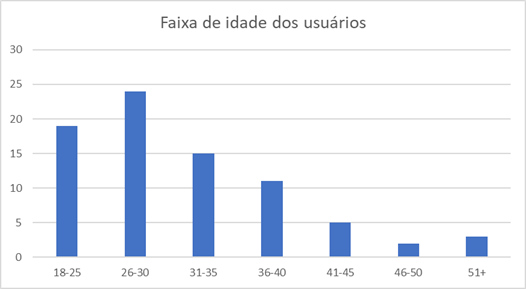
\includegraphics[width=0.6\linewidth]{images/distribuicao-idade.png}\\
  \end{center}
  \caption[Distribuição de faixa etária]{Distribuição de faixa etária}
  \label{fig:mapa-empatia=inicial}
  \legend{Fonte: Próprio Autor}
\end{figure}

A segunda pergunta foi quanto a localidade (estado) em que o entrevistado mora. Pelo gráfico abaixo, podemos ver que a maior parte dos entrevistados foram oriundos do estado de São Paulo. Embora a pesquisa não tenha conseguido coletar dados e pessoas de alguns estados, podemos ver que conseguimos abranger uma boa parte dos estados brasileiros.
\begin{figure}[H]
  \begin{center}
  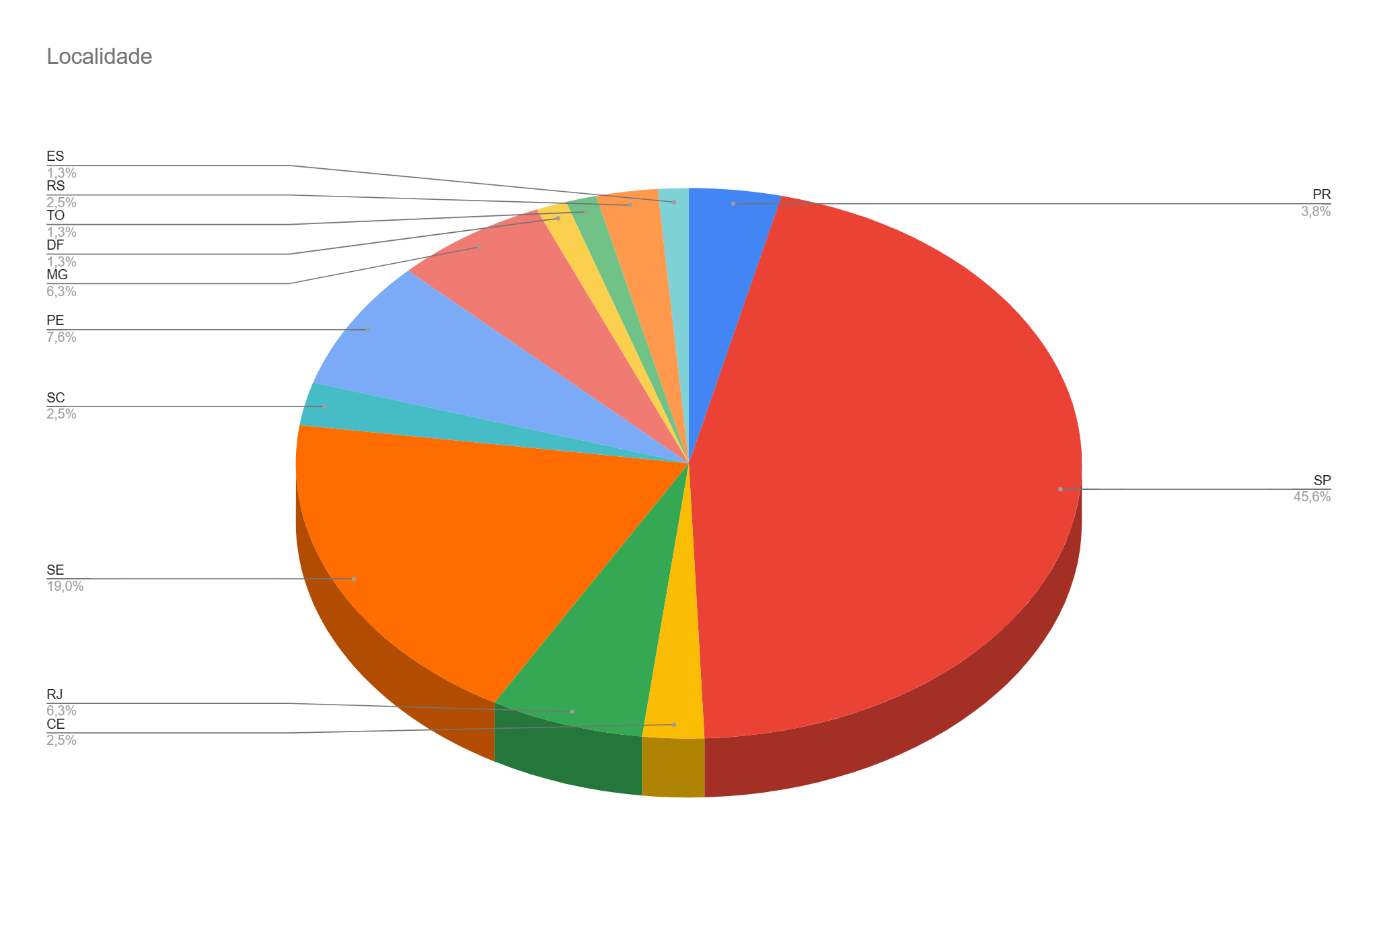
\includegraphics[width=0.6\linewidth]{images/distribuicao-estados.png}\\
  \end{center}
  \caption[Distribuição de localização]{Distribuição de localização}
  \label{fig:mapa-empatia=inicial}
  \legend{Fonte: Próprio Autor}
\end{figure}

\subsection{Segurança}
A primeira pergunta relacionada a segurança foi quanto ao fato do entrevistado se privar de ir a lugares por conta de ser uma mulher. O gráfico abaixo nos mostra, que infelizmente, muitas mulheres ainda se privam de ir a determinados lugares por conta do medo do que pode acontecer a elas, simplesmente por serem mulheres. 
\begin{figure}[H]
  \begin{center}
  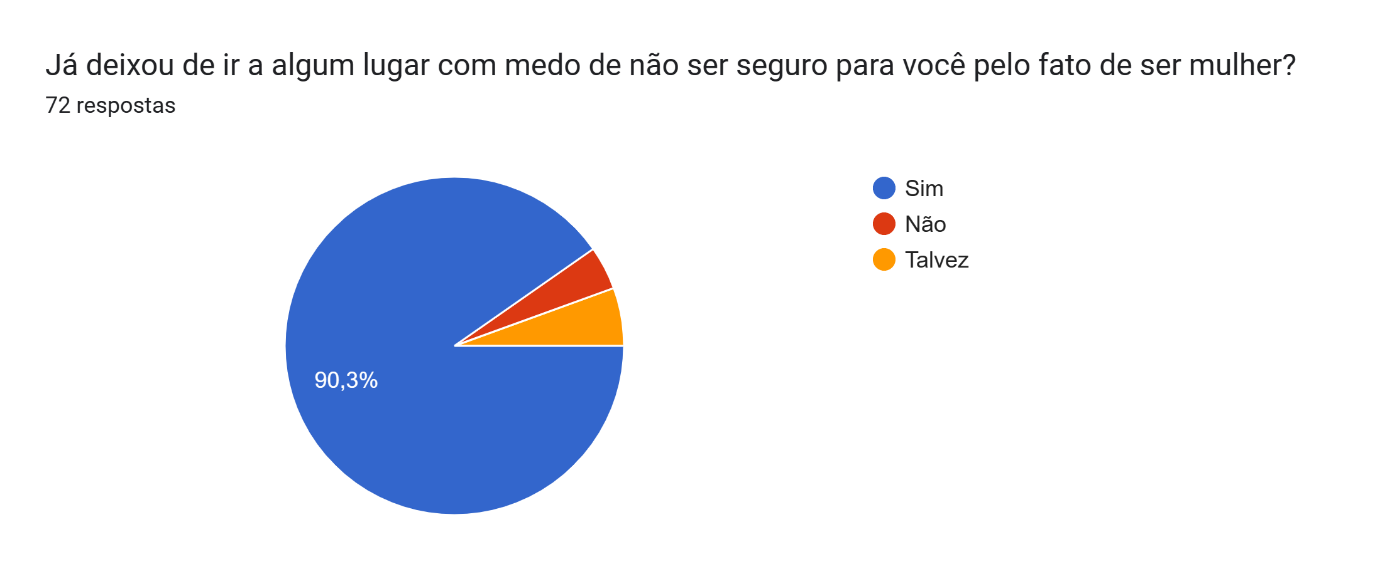
\includegraphics[width=1.0\linewidth]{images/distribuicao-privacao-mulher.png}\\
  \end{center}
  \caption[Distribuição de privação de local]{Distribuição de privação de local}
  \label{fig:mapa-empatia=inicial}
  \legend{Fonte: Próprio Autor}
\end{figure}
%\clearpage

A segunda pergunta foi sobre o entrevistado se sentir seguro ao andar na rua. O resultado abaixo nos mostra que majoritariamente as mulheres não se sentem seguras ao andar na rua. Tendo o receio de andar na rua em determinados lugares. 
\begin{figure}[H]
  \begin{center}
  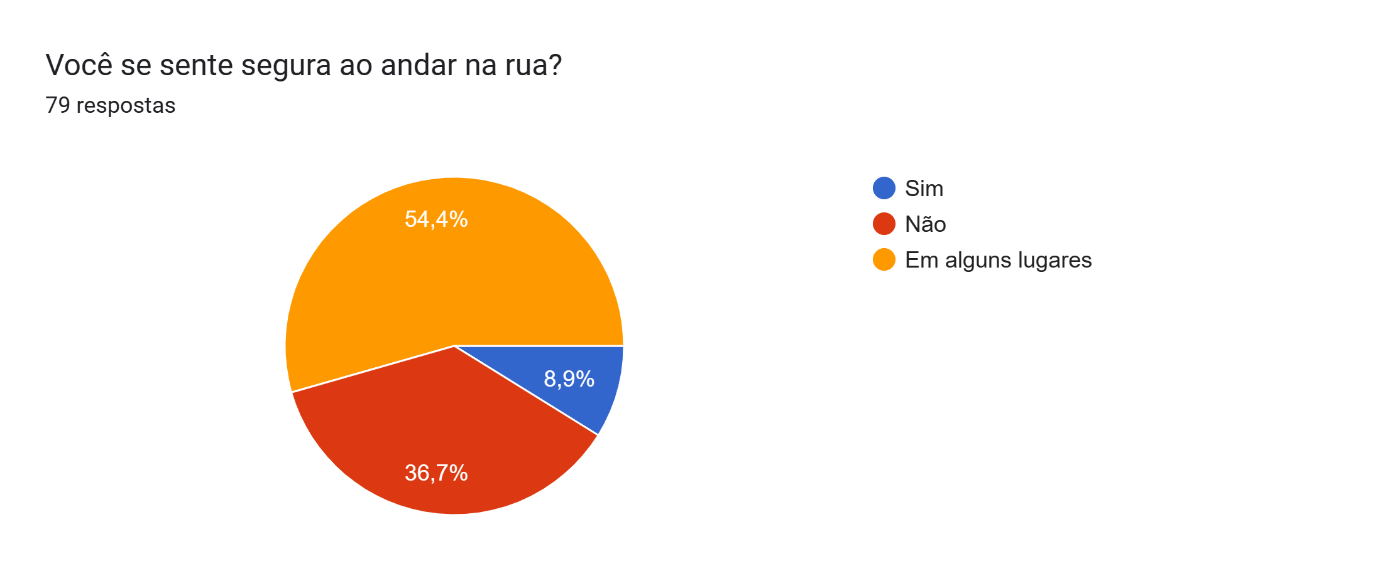
\includegraphics[width=1.0\linewidth]{images/distribuicao-seguranca-rua.png}\\
  \end{center}
  \caption[Distribuição de sentimento de segurança]{Distribuição de sentimento de segurança}
  \label{fig:mapa-empatia=inicial}
  \legend{Fonte: Próprio Autor}
\end{figure}
%\clearpage

A terceira pergunta desta seção foi relacionada ao tipo de medo que a mulher sentia ao sair à noite sozinha. A pergunta poderia ter várias respostas escolhidas e os resultados abaixo nos mostram que a violência ainda continua sendo o principal medo reportado por elas.
\begin{figure}[H]
  \begin{center}
  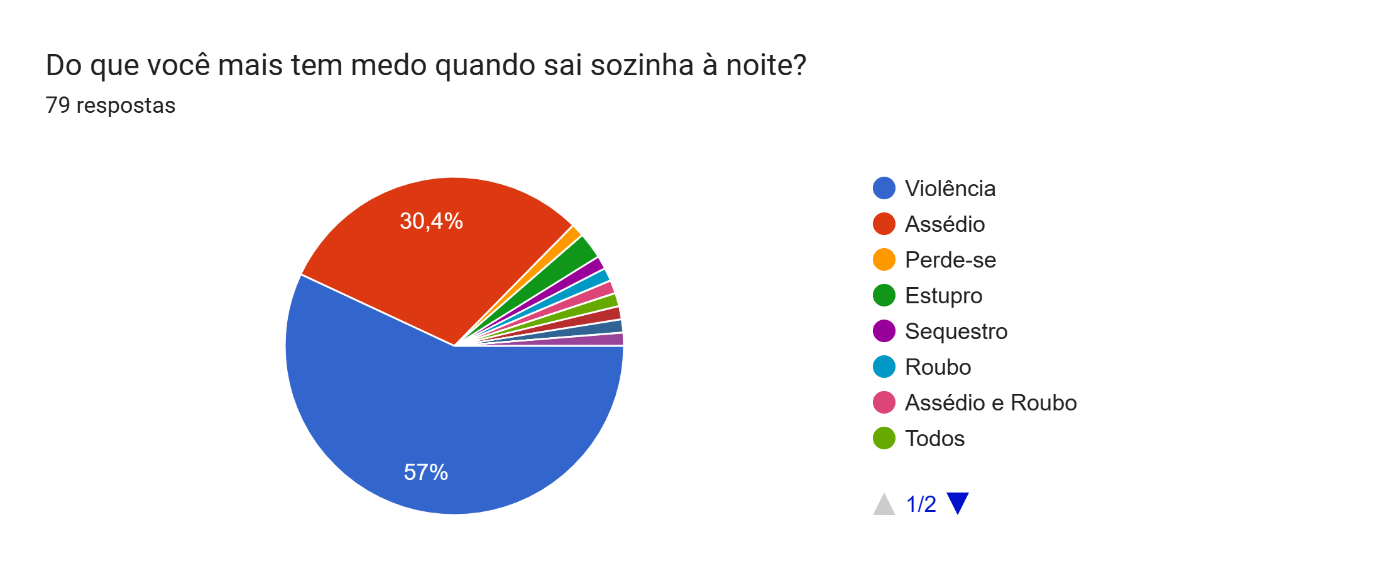
\includegraphics[width=0.5\linewidth]{images/distribuicao-medo.png}\\
  \end{center}
  \caption[Distribuição de maior medo]{Distribuição de maior medo}
  \label{fig:mapa-empatia=inicial}
  \legend{Fonte: Próprio Autor}
\end{figure}
%\clearpage

A última pergunta da seção de segurança foi um pouco mais direta quanto ao fato da entrevistada já ter sofrido algum tipo de violência ou assédio. Mais uma vez, majoritariamente, podemos ver que infelizmente muitas mulheres já passaram por essas situações. 
\begin{figure}[H]
  %\begin{center}
  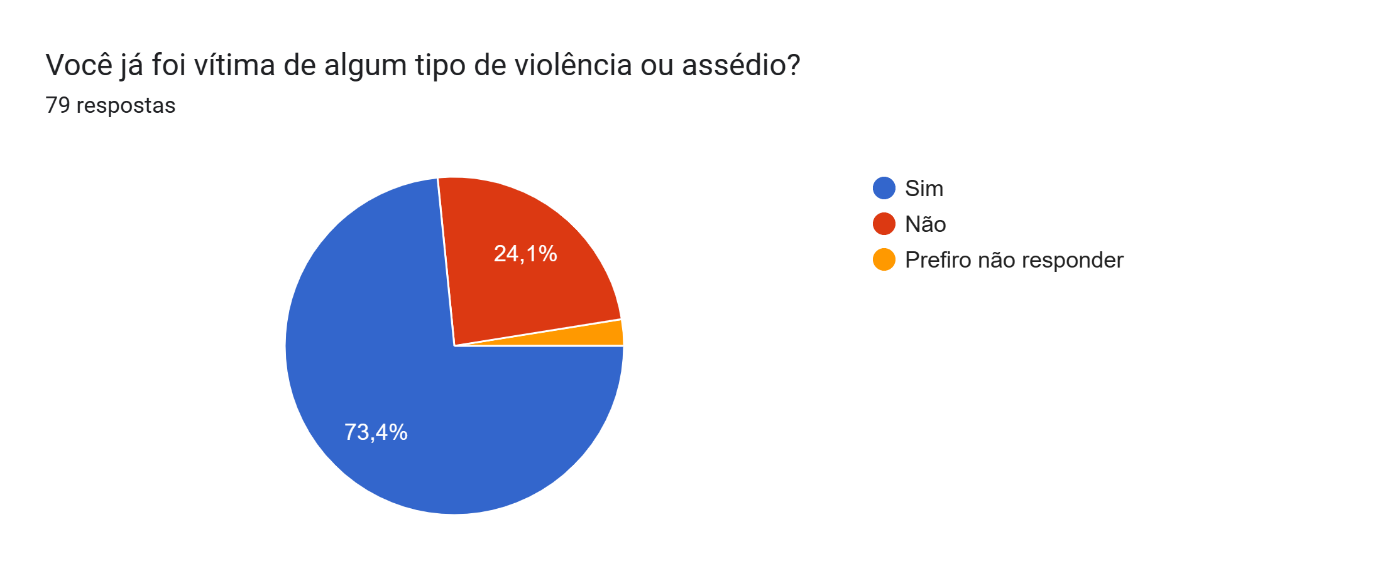
\includegraphics[width=0.5\linewidth]{images/distribuicao-vitma.png}\\
  %\end{center}
  \caption[Distribuição de vítima]{Distribuição de vítima}
  \label{fig:distribuicao-vitmal}
  \legend{Fonte: Próprio Autor}
\end{figure}
%\clearpage

\subsection{Uso do aplicativo}
A primeira pergunta nesta seção indagava aos entrevistados sobre o uso de um aplicativo capaz de mostrar informações sobre a segurança de um determinado local. Abaixo podemos ver no gráfico que os usuários percebem a utilidade em usar um aplicativo para tal fim.

\begin{figure}[h]
  \begin{center}
  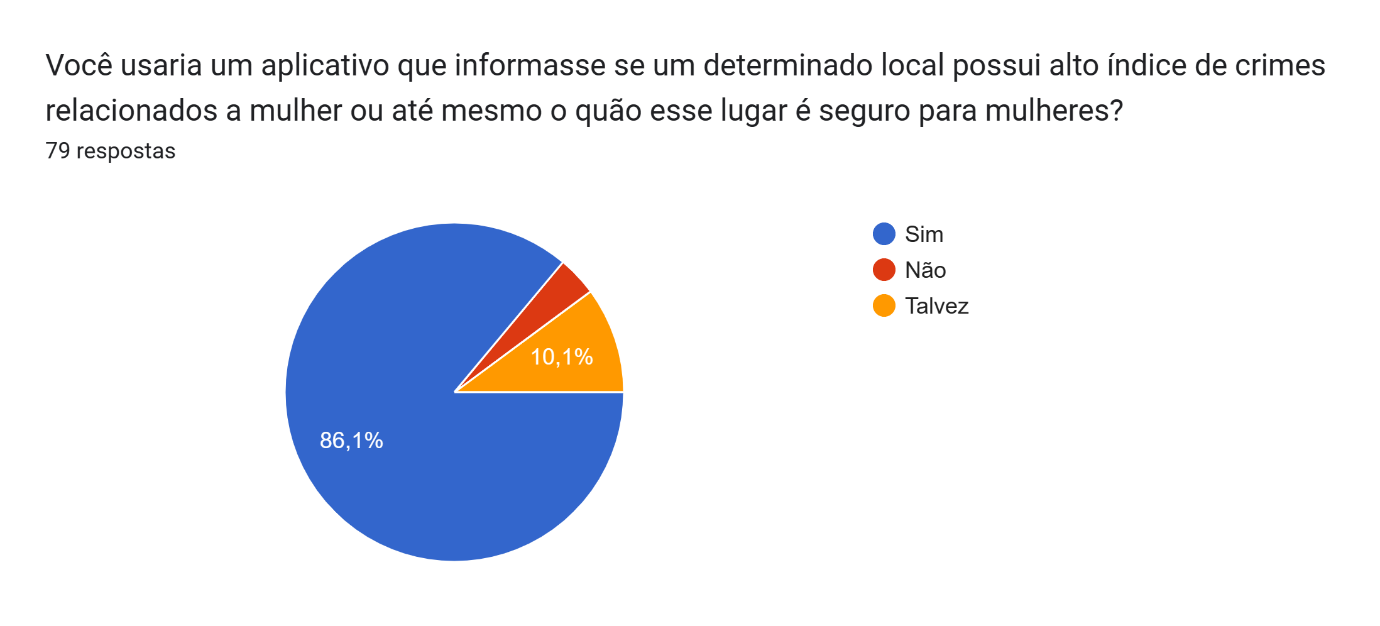
\includegraphics[width=1.0\linewidth]{images/distribuicao-uso-aplicativo.png}\\
  \end{center}
  \caption[Distribuição uso do aplicativo]{Distribuição uso do aplicativo}
  \label{fig:distribuicao-uso-aplicativo}
  \legend{Fonte: Próprio Autor}
\end{figure}

A segunda pergunta nesta seção focava sobre quais as funcionalidades que os usuários gostariam de ver no aplicativo. Abaixo é mostrado um resumo das escolhas dos usuários onde é possível notar que informações sobre segurança, forma de pedir ajuda e rastreamento em tempo real foram as funcionalidades mais votadas. As opções de respostas eram:
\begin{itemize}
  \item Informações sobre segurança do local
  \item Possibilidade de pedir ajuda em caso de emergência
  \item Rastreamento de localização
  \item Rede de apoio com outras mulheres
  \item Outros
\end{itemize}

\begin{figure}[h]
  \begin{center}
  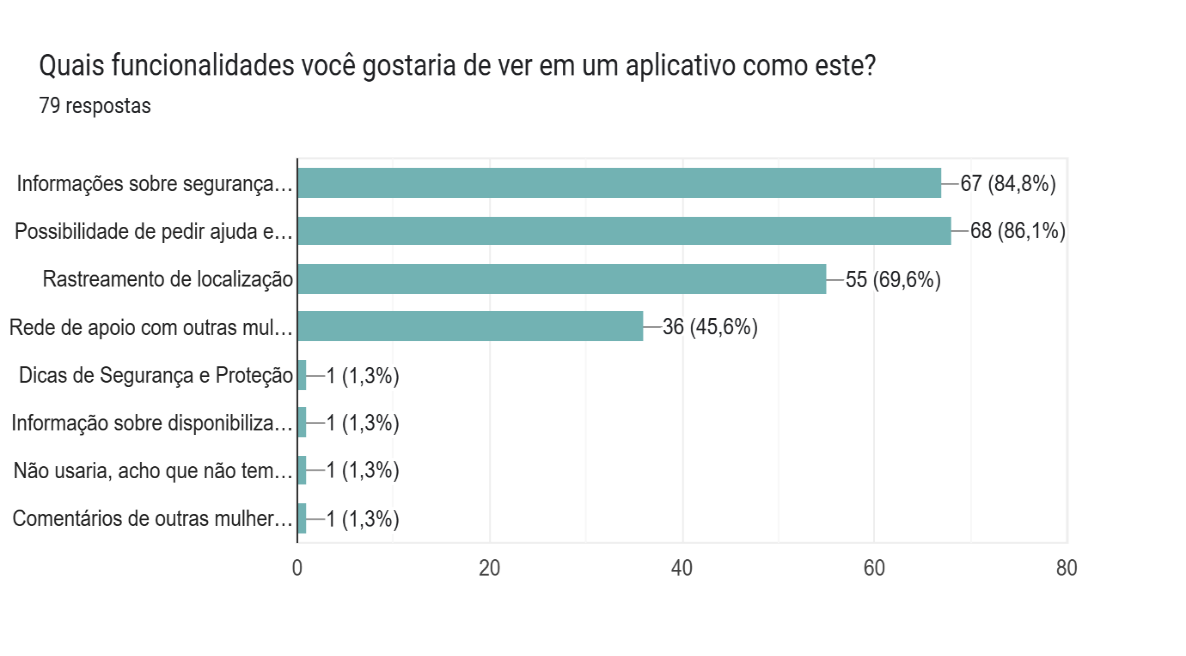
\includegraphics[width=1.0\linewidth]{images/distribuicao-escolha-funcionalidades.png}\\
  \end{center}
  \caption[Distribuição de escolha de funcionalidades]{Distribuição de escolha de funcionaldades}
  \label{fig:distribuicao-escolha-funcionalidades}
  \legend{Fonte: Próprio Autor}
\end{figure}

\subsection{Comentários gerais}
Foi adicionada uma seção em que os entrevistados podiam deixar suas opiniões e sugestões. Dando foco emalgumas opniões que foram relatas, foi possível perceber certas preocupações dos possíveis usuários do aplicativo. 

Um entrevistado escreveu o seguinte comentário: “Minha preocupação seria na possibilidade de criminosos utilizarem o aplicativo para terem acesso a essas mulheres, dependendo do tipo de funcionalidade implementada”. Realmente ao mesmo tempo em que temos que nos preocupar em disponibilizar uma ferramenta para ajudar nossos usuários, temos que garantir a segurança desta ferramenta, para que ela não acabe se tornando uma arma para criminosos.

Outro entrevistado escreveu: “Talvez informar que o local é inseguro nos traz mais insegurança do que o necessário. Muitas podem desencadear reações ruins como síndrome do pânico e ansiedade, até depressão e se isolar (não sou especialista), mas, por exemplo, deixo de assistir noticiários por excesso de notícias ruins nos deixar em pânico.”. A intenção é que a aplicação possa ajudar nossos usuários à terem menos receio quanto a segurança. A ideia de implementar um histórico sobre local ou até mesmo índice de criminalidade terá que ser amadurecida.

“Acredito que será de grande utilidade para levantamento de dados para a segurança pública, mas a maioria das vezes, a mulher TEM que ir ao lugar independente da informação... então não vejo um avanço significativo para a mulher diretamente, seria mais para levantamento de dados da segurança pública mesmo.” A fala desta entrevistada demonstra como hoje ainda há muito da cultura patriarcal. A intenção da ferramenta não é dizer aonde nosso usuário deve ir ou não, mas sim mostrar dados acerca da segurança de um determinado local. Este comentário corrobora com o comentário anterior sobre acabar criando algum tipo de síndrome no nosso usuário.

\section{Novo Personas e Mapa de empatia}
Dadas as informações coletadas podemos verificar que nossas suposições do mapa de empatia foram validadas em sua maior parte. Desta forma, alguns pontos puderam ser levantados e mapeados em um novo mapa muito parecido com o primeiro, porém contendo agora algumas entradas mais voltadas ao problema. Abaixo podemos ver os novos pontos adicionados ao nosso mapa de empatia.
\begin{figure}[h]
  \begin{center}
  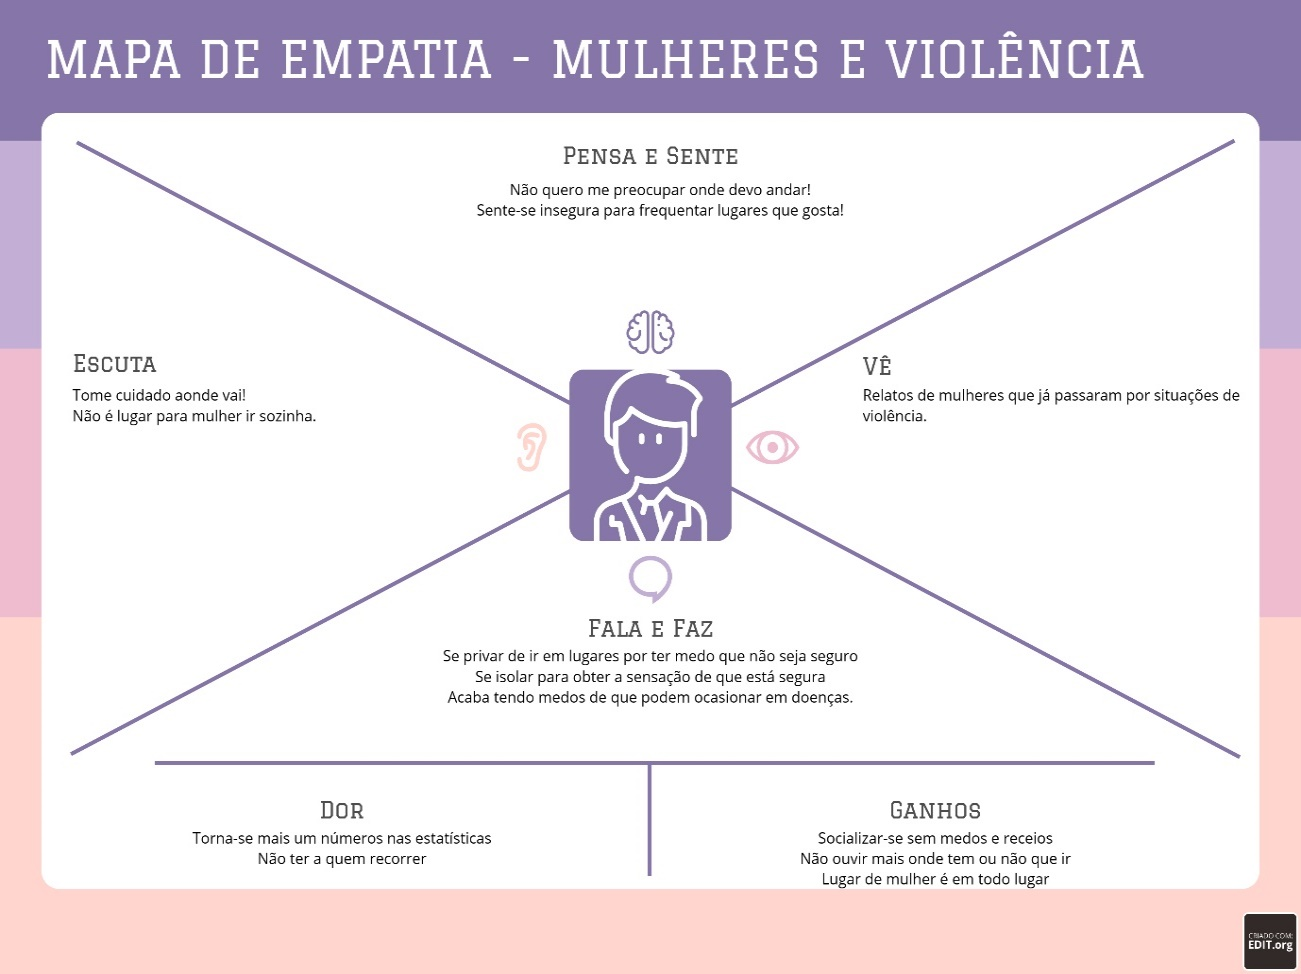
\includegraphics[width=1.0\linewidth]{images/mapa-empatia-novo.jpeg}\\
  \end{center}
  \caption[Nobo mapa de mepatia]{Novo mapa de empatia}
  \label{fig:novo-mapa-empatia}
  \legend{Fonte: Próprio Autor}
\end{figure}

Quanto ao nosso novo personas podemos agora enfatizar alguns pontos que antes não haviam ainda sido vistos em nossa análise.

Persona: Pessoas do sexo feminino de qualquer idade que em algum momento da vida já teve receio de sair de casa por medo da violência que pode ocorrer contra ela. São mulheres que desejam ter uma forma de pedir ajuda quando alguma situação estranha ou adversa estiver acontecendo com elas. São mulheres que não se sentem seguras ao sair de casa sozinha, pois acreditam que algo pode acontecer contra elas e não terão como pedir ajuda. Essas mulheres utilizam seus celulares no dia a dia para fazerem ligações, conversar por aplicativos de mensagens instantâneas e as até para pedir ajuda a pessoas as quais ela considera confiáveis. Em casos extremos, são mulheres que já sofreram ou sofrem algum tipo de violência, seja ela doméstica, verbal, moral ou até mesmo física e que não tem ou tinham, quando o ato ocorreu, uma forma de requisitar ajuda as pessoas a qual ela confia.


\chapter{Princípios de Usabilidade}

Os princípios de design e os princípios de usabilidade constituem os fundamentos teóricos e práticos essenciais para o desenvolvimento de interfaces de usuário eficazes e experiências digitais significativas. Em um cenário onde as expectativas dos usuários evoluem continuamente e as tecnologias digitais se tornam cada vez mais complexas, a compreensão e aplicação adequada destes princípios torna-se crucial para o sucesso de produtos digitais.


\section{Princípios de usabilidade}

A usabilidade refere-se à medição de quão facilmente um usuário pode alcançar seus objetivos ao usar um serviço \cite{digital_gov_usability}. Isso geralmente é medido através de metodologias de pesquisa estabelecidas sob o termo "teste de usabilidade", que inclui taxas de sucesso e satisfação do cliente. A usabilidade é uma parte do guarda-chuva mais amplo da experiência do usuário (UX). Enquanto UX abrange o design da experiência geral de um produto, a usabilidade foca na mecânica de garantir que os produtos funcionem da melhor forma possível para o usuário.
\begin{comment}
Doze princípios de usabilidade padrão da indústria são usados para avaliar formalmente a usabilidade de sistemas, aplicações e interfaces \cite{stanford_usability}. Estes princípios são informados por várias diretrizes de usabilidade da indústria, incluindo princípios consistentes que nos permitem alinhar melhor aos padrões aprimorados para experiência do usuário.

	Este capítulo introduz os fundamentos do design para usabilidade e UX, focando na aplicação de ciência, arte e artesanato ao seu design fundamentado \cite{researchgate_usability_ux}. Ele revisa os principais métodos de avaliação de usabilidade, focando em testes de usabilidade. O conceito de UX lança uma rede ampla sobre todas as experiências do usuário.
\end{comment}

Em 2024, o tema "Designing for a Better World" com foco em usabilidade, sustentabilidade e inclusividade pôde ser visto em vários contextos \cite{world_usability_day}. Esta abordagem contemporânea reflete a crescente consciência sobre a responsabilidade social do design e a necessidade de criar soluções que não apenas funcionem bem, mas também contribuam positivamente para a sociedade.

Os designers são encorajados a se manterem atualizados com estes princípios para atender às expectativas evolutivas dos usuários e entregar soluções digitais impactantes \cite{medium_ui_principles_2025}. A evolução contínua da tecnologia e das expectativas dos usuários requer uma abordagem dinâmica à aplicação de princípios de design e usabilidade.

\section{Princípios de design}

Os princípios de design referem-se aos fundamentos teóricos e diretrizes práticas que orientam a criação de interfaces visuais e funcionais eficazes. Em 2024, o design de interface de usuário (UI) enfatiza princípios como design centrado no usuário, acessibilidade e simplicidade para aprimorar experiências digitais \cite{slideshare_ui_principles_2024}. As principais tendências também incluem design responsivo, micro-interações e a integração de personalização e design de movimento para criar interfaces envolventes e sustentáveis.

O design de interface de usuário bem-sucedido torna-se mais fácil quando você compreende os 14 princípios fundamentais de design de UI, começando pelo design para o usuário \cite{uxpin_ui_principles}. Estes princípios fornecem uma estrutura conceitual que permite aos designers tomarem decisões informadas e criarem soluções que atendam tanto às necessidades funcionais quanto às expectativas estéticas dos usuários.
\begin{comment}
	Como designer de UX, você deve priorizar a usabilidade sobre a estética. Incorpore testes de usabilidade no processo de design para identificar (e corrigir) problemas de usabilidade, garantindo uma experiência do usuário amigável e eficiente em geral \cite{ux_design_institute}. Os sete princípios de UX design devem ser mantidos em mente para alcançar resultados efetivos.
\end{comment}

Muitos designers e educadores de Interface de Usuário (UI) discutem princípios a serem seguidos ao projetar os aspectos funcionais de uma UI \cite{tandfonline_ui_principles}. No entanto, muitos princípios de UI foram propostos, espalhados na literatura científica, criando a necessidade de uma abordagem unificada para a compreensão e aplicação destes conceitos.

\section{Usabilidade SheSafe}
\begin{comment}
	Você tem que deixar claro que essas telas fazem parte do projeto inicial e que procurou colocar elementos nas telas de modo a atender os princípios de usabilidade, mas não precisa ficar dizendo qual é qual.
\end{comment}
A seguir é possível ver as telas que fazem parte do wireframe do projeto inicial da interface. Nas telas foram inseridos elementos que atendem aos princípios de usabilidae e os reforçam.
\subsection{Tela 1 - Home}
\begin{figure}[h]
  \begin{center}
  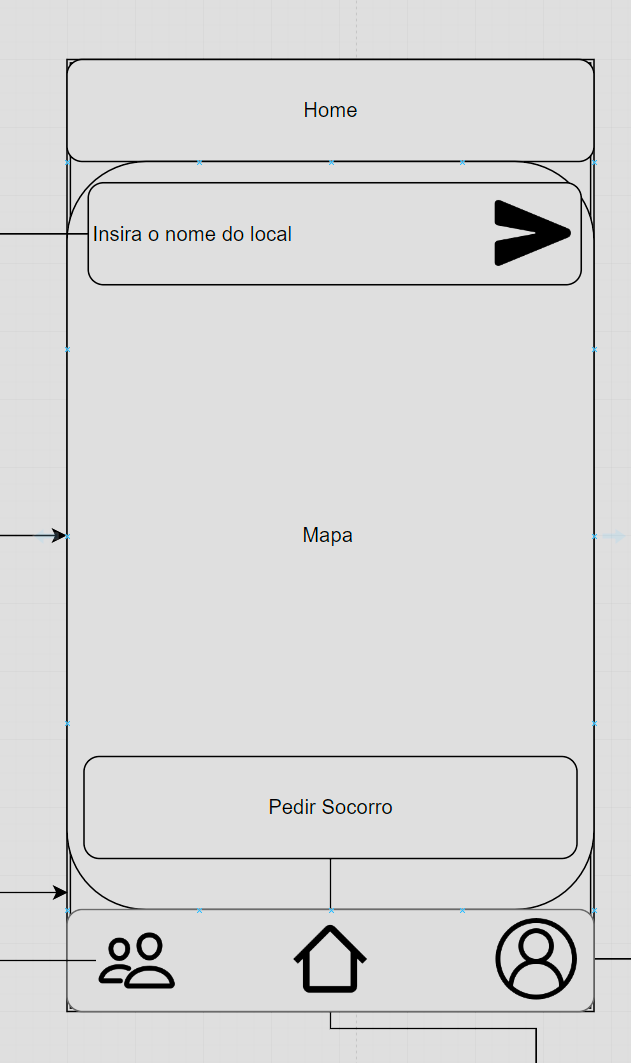
\includegraphics[width=0.2\linewidth]{images/wire-tela-home.png}\\
  \end{center}
  \caption[Wireframe Tela Home]{Wireframe Tela Home}
  \label{fig:wireframe-tela-home}
  \legend{Fonte: Próprio Autor}
\end{figure}
\pagebreak
\begin{comment}
	\begin{alineas}
		\item Tipo de interface e interação
		
		Na tela home será utilizada o tipo de tela de interface gráfica onde o usuário irá visualizar sua localização atual no mapa e um campo de busca e um botão de pedido de socorro. A forma de interação será através de toque nos botões tanto da bottom bar quanto do pedir socorro. E através de formulário no campo para inserir o nome do local a ser buscado.
		\item Metáforas
		
		A BottomBar contém ícones os quais remetem as funcionalidades do aplicativo. O ícone com dois bonecos remete a uma lista de contatos. O ícone da casa remete a tela principal de qualquer aplicativo. Já o ícone circular com boneco dentro remete ao perfil em qualquer aplicação. A própria BottomBar já remete a ideia de que é possível navegar entre essas três telas sem que tenha que sair deste menu em si. 
		\item Aprendizibilidade
		
		Previsibilidade – Ao clicar em qualquer um dos ícones da bottom bar o usuário será navegado para a tela correspondente ao ícone.
		
		Capacidade de sintetização – O usuário receberá um alert em formato de notificação Toast ao clicar em enviar pedido de socorro e confirmar (caso a confirmação de envio esteja ativada) que deseja enviar.
		
		Familiaridade – Não se aplica.
		
		Consistência – A bottom bar será apresentada sempre no fim das três telas principais (contatos, home e perfil). E os seus ícones estarão sempre na mesma ordem de posição.
		
		Generalização – Não se aplica.
		\item Flexibilidade
		
		Iniciativa de diálogo – É possível cancelar o pedido de socorro ao clicar em cancelar (caso a confirmação de envio esteja ativada).
		
		Multitarefa – Não se aplica.
		
		Migração de atividades – Não se aplica.
		
		Substitutividade – Não se aplica.
		
		Personalização – Não se aplica.
		\item Robustez
		
		Observabilidade – O mapa indicará a localização atual do usuário na tela home.
		
		Recuperabilidade – O sistema irá emitir um alert em formato de Toast indicando quando houver falha no envio de um pedido de socorro e pedirá para que o usuário refaça a solicitação.
		
		Capacidade de resposta – Ao enviar ou confirmar um pedido de socorro o sistema irá emitir um alerta em formato de Toast indicando que o pedido foi enviado.
		
		Conformidade de realização de atividades – O usuário irá receber na tela um aviso em caso de perda de conexão e pedirá que o usuário se reconecte antes de continuar as operações. 
	\end{alineas}
\end{comment}
Na tela home será utilizada a interface gráfica onde será possível o usuário visualizar um mapa com sua localização atual. Haverá um campo de busca e um botão para acionamento do pedido de socorro. Toda a interação será realizada através de toque nos botões da bottom bar, no botão de pedido de socorro e no formulário de busca.

A bottom bar conterá três ícones que represetam as funcionalidade principais do aplicativo. O ícone com dois bonecos remete a lsita de contatos. O ícone da casa remete a tela principal nos aplicativos que utilizam tal ícone. Já o ícone circular com boneco remete ao perfil nos aplicativos em que é utilizado. A própri abottom bar já consiste na idea de uma interface navegável entre as três funcionalidade principais do aplicativo. Cada ícone ao ser clicado, deverá navegar para tela correspondente ao ícone.

A bottom bar estará posicionada sempre no fim da tela das três telas principais(contatos, home e perfil), contendo smepre os mesmos ícones e o mesmo posicionamento mantendo assim a sua consistência

Será enviado aum alert em formato de notificação Toast após o acionamento do botão de pedido de socoroo e sua confirmação(caso esteja ativada a confirmação de envio). Uma notificação Toast também será enviada caso o envio do pedido de socorro resultar em uma falha. 

Será possível cancelar o pedido de socorro ao clicar em cancelar(caso a confirmação de envio esteja ativada) no dialog de confirmação que será apresentado. 

\subsection{Tela 2 - Local}
\begin{figure}[h]
  \begin{center}
  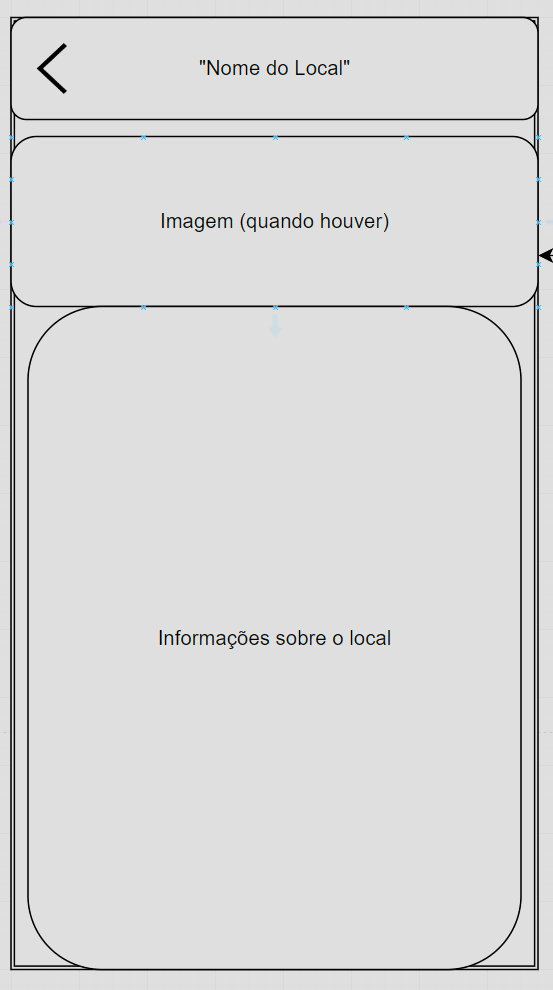
\includegraphics[width=0.2\linewidth]{images/wire-tela-local.png}\\
  \end{center}
  \caption[Wireframe Tela Local]{Wireframe Tela Local}
  \label{fig:wireframe-tela-local}
  \legend{Fonte: Próprio Autor}
\end{figure}
Na tela local será possível visualizar na tela a imagem de um determinado local buscado(quando houve) sempre na parte superior da tela acima das informação em formato de texto. 

Haverá uma app bar onde o título deverá apresentar o nome do local. Essa app bar estará posicionada sempre no início da tela. Ela conterá um ícone de seta virada para esquerdade que remete a ação de voltar a tela nos aplicativos.
\begin{comment}
\begin{alineas}
  \item Tipo de interface e interação
  
Na tela lugar será utilizada o tipo de tela de interface gráfica onde o usuário irá visualizar informações sobre o local que ele clicou na tela home. A forma de interação será através de toque no botão de voltar para retroceder a tela home. 
  \item Metáforas
  
Ícone de seta para esquerda indicando a ação de voltar na tela. O ícone estará presente no toolbar da tela no canto superior esquerdo como é de costume em aplicações mobile.
  \item Aprendizibilidade
  
Previsibilidade – Ao clicar no ícone da seta para esquerda espera-se que retroceda uma tela.

Capacidade de sintetização – Não se aplica.

Familiaridade – Não se aplica.

Consistência – O ícone de voltar aparecerá sempre no mesmo local, ou seja, canto superior esquerdo.

Generalização – Não se aplica.

  \item Flexibilidade
  
Iniciativa de diálogo – Não se aplica.

Multitarefa – Não se aplica.

Substitutividade – Não se aplica.

Personalização – Não se aplica.


  \item Robustez
  
 Observabilidade – Os dados apresentados na tela serão do local escolhido na busca na tela anterior.
 
Recuperabilidade – O sistema irá emitir um alert em formato de Toast indicando quando houver falha no envio de um pedido de socorro e pedirá para que o usuário refaça a solicitação.

Capacidade de resposta – Não se aplica.

Conformidade de realização de atividades – Não se aplica. 
\end{alineas}
\end{comment}
\subsection{Tela 3 - Perfil}
\begin{figure}[h]
  \begin{center}
  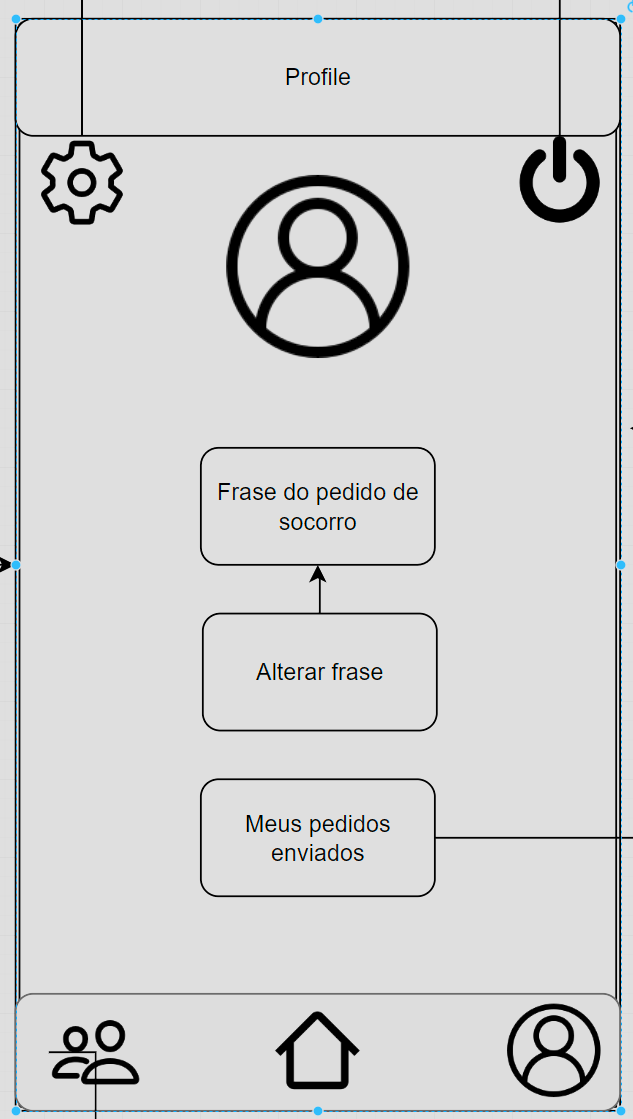
\includegraphics[width=0.2\linewidth]{images/wire-tela-perfil.png}\\
  \end{center}
  \caption[Wireframe Tela Perfil]{Wireframe Tela Perfil}
  \label{fig:wireframe-tela-perfil}
  \legend{Fonte: Próprio Autor}
\end{figure}
\pagebreak
O título da tela será sempre apresentado no início da tela.  Na tela de perfil será apresentado dois icone um de engrenagem que remete ao acesso a área de configurações em qualquer aplicativo e também o ícone de power off que remete a ação de logar/deslogar de qualquer aplicativo. 

Abaixo do título da tela será exibida a imagem de perfil do usuário(quando houver) ou um ícone padrão de perfil(quando não houver).

Será exibido a frase do pedido se soccoro(frase padrão até ser editada pelo usuário) a ser enviada e apresentado um botão para acionamento da edição desta frase para um texto pessoal definido pelo usuário. 

Abaixo da frase será exibido os ultimos pedidos de socorro enviados ou um frase de alert no caso de nenhum pedido tenha sido enviado. Nesta mesma área será possível acionar através de toque um botão que levará o usuário para a ela onde poderá acessar todos os pedidos que ele já enviou visto que nesta tela serão apresenados apenas os últimos pedidos.
\begin{comment}
\begin{alineas}
  \item Tipo de interface e interação
  
Na tela de perfil será utilizada o tipo de tela de interface gráfica com multi toque. A forma de interação será através de multi toque, onde ao clicar nas opções disponíveis na tela será possível realizar a ação correspondente. 
  \item Metáforas
  
A BottomBar contém ícones os quais remetem as funcionalidades do aplicativo. O ícone com dois bonecos remete a uma lista de contatos. O ícone da casa remete a tela principal de qualquer aplicativo. Já o ícone circular com boneco dentro remete ao perfil em qualquer aplicação. A própria BottomBar já remete a ideia de que é possível navegar entre essas três telas sem que tenha que sair deste menu em si. Há também dois botões de ícones que indicam configurações(engrenagem) e logoff(power).
  \item Aprendizibilidade
  
Previsibilidade – Ao alterar a mensagem do pedido de socorro o usuário recebe um alert em forma de Toast indicando que a alteração foi concluída com sucesso. 

Capacidade de sintetização – Após alterar a mensagem de pedido de socorro a nova mensagem é automaticamente exibida na área da tela onde a mensagem é mostrada.

Familiaridade – Não se aplica.

Consistência – Após a alteração da mensagem de pedido de socorro, os novos pedidos enviados devem ser emitidos com a nova mensagem. Não há alterações para os pedidos já enviados anteriormente.

Generalização – Não se aplica.

  \item Flexibilidade
  
Iniciativa de diálogo – Não se aplica.

Multitarefa – Não se aplica.

Migração de atividades – Caso o usuário altere a mensagem e não clique em salvar, ao sair do foco do campo de inserir a mensagem, o conteúdo atual é salvo como nova mensagem.

Substitutividade – Não se aplica.

  \item Robustez
  
Observabilidade – O usuário irá ver automaticamente a nova mensagem de pedido de socorro assim que ele salvar a sua edição.

Recuperabilidade – Não se aplica.

Capacidade de resposta – Não se aplica.

Conformidade de realização de atividades – Não se aplica

\end{alineas}
\end{comment}
\subsection{Tela 4 - Configurações}
\begin{figure}[h]
  \begin{center}
  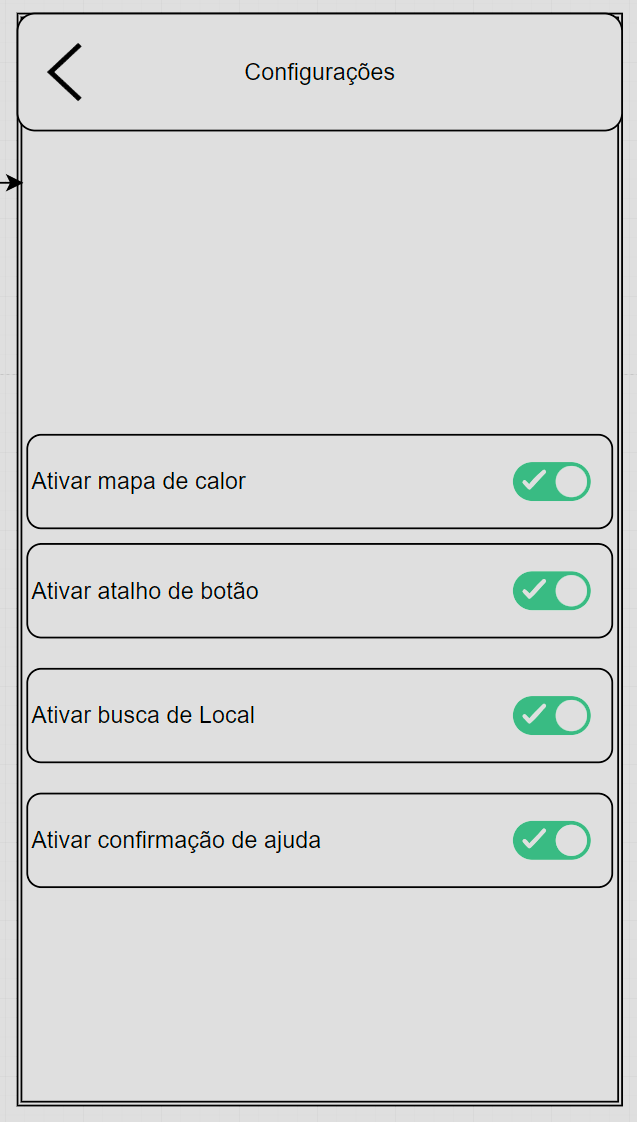
\includegraphics[width=0.2\linewidth]{images/wire-tela-configuracoes.png}\\
  \end{center}
  \caption[Wireframe Tela Configurações]{Wireframe Tela Configurações}
  \label{fig:wireframe-tela-configuracoes}
  \legend{Fonte: Próprio Autor}
\end{figure}
\pagebreak
Na tela de configurações serão apresentadas as customizações que serão possíveis realizar no aplicativo. Através de switch toggles, que remete a liga e desliga, o usuário será capaz de ativar ou desativar as customizações possíveis da aplicação. O usuário poderá realizar o acionamento do switch através de clique ou através de gesto de arrastar a chave para a nova posição.
\begin{comment}
\begin{alineas}
  \item Tipo de interface e interação
  
O tipo de interface será de central de controle, onde o usuário será capaz de ativar ou desativar alguns recursos e configurações do aplicativo. 
A interação será através de gesto de deslize para ativar ou desativar as chaves para cada configuração presente na tela.

  \item Metáforas
  
Os toggles dão ideia de um interruptor para desligar ou ligar a configuração respectiva.
  \item Aprendizibilidade
  
Previsibilidade – Ao acionar o toggle o sistema emitirá alertas de que a respectiva funcionalidade foi liga ou desligada.

Capacidade de sintetização – Não se aplica.

Familiaridade – Os toggle remetem ao interruptor da vida real. 

Consistência – Não se aplica.

Generalização – Não se aplica.

  \item Flexibilidade
  
Iniciativa de diálogo – Não se aplica.

Multitarefa – Não se aplica.

Migração de atividades – Não se aplica.

Substitutividade – Não se aplica.

Personalização – Não se aplica.

  \item Robustez
  
Observabilidade – Ao acionar o toggle de alguma das funcionalidades o usuário será capaz de ver imediatamente o novo estado desta funcionalidade, se está ativada ou não.

Recuperabilidade – Não se aplica.

Capacidade de resposta – Um alert em formato Toast será exibido cada vez em que o estado de uma das funcionalidades for alterado entre liga e desliga.

Conformidade de realização de atividades – Não se aplica
\end{alineas}
\end{comment}
\subsection{Tela 5 - Tela Cadastro contato seguro}
\begin{figure}[h]
  \begin{center}
  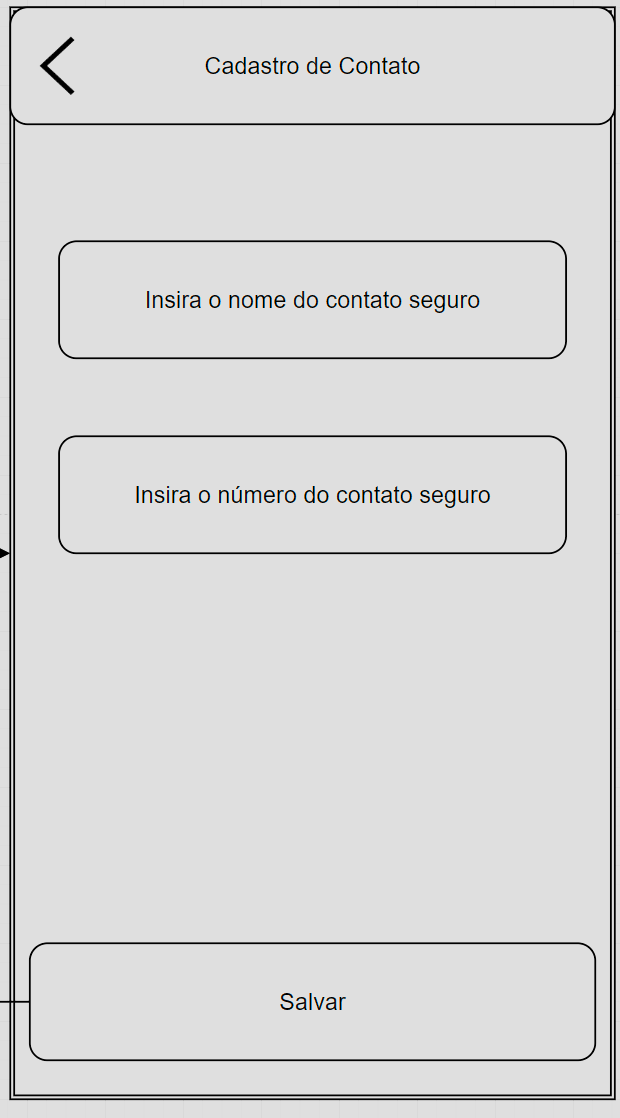
\includegraphics[width=0.2\linewidth]{images/wire-tela-cadsatro-contato-seguro.png}\\
  \end{center}
  \caption[Wireframe Tela Cadastro contato seguro]{Wireframe Tela Cadastro contato seguro}
  \label{fig:wireframe-tela-cadastro-contato-seguro}
  \legend{Fonte: Próprio Autor}
\end{figure}
\pagebreak
Será apresentado um formulário onde o usuário será capaz de inserir os dados do seu contato seguro. Para interação com o formulário o usuário deverá clicar em cada um dos campos para inserção dos dados. Alertas de erros nos campos serão exibidos quando o usuário tentar enviar o formulário com dados inválidos(formulário com dados vazios, dígitos no campo de nome). 

Através do botão salvar os dados serão enviados para cadastramento na base de dados. Será exibidada um tela de carregamento enquanto os dados estirevem em transferência para base de dados, mantendo assim o usuário informado sobre a sua ação de salvamento. O mesmo formulário também será utilizado para edição do contato seguro. Neste cenário as dados do cadastro já viram preenchidos e o usuário poderá alterar tais dados.

Através do ícone da seta para a esquerda, assim como nas outras telas em que aparece, o usuário será capaz de retornar a tela anterior. 
\begin{comment}
\begin{alineas}
  \item Tipo de interface e interação
  
A interface será do tipo formulário onde o usuário deverá preencher os dados para cadastro do contato seguro. O tipo de interação será através de preenchimento de campos.
  \item Metáforas
  
Um botão com ícone de seta para esquerda será exibido na app bar indicando a ação de voltar para tela anterior.
  \item Aprendizibilidade
  
Previsibilidade – Um alert em forma de Toast será exibido ao salvar com sucesso um contato.

Capacidade de sintetização – Ao salvar o novo contato com sucesso a tela de listagem de contatos deverá exibir a listagem já com o novo contato inserido na tela. 

Familiaridade – O contato seguro remete a um contato de telefone na agenda do usuário.

Consistência – Não se aplica.

Generalização – Não se aplica
  \item Flexibilidade
  
Iniciativa de diálogo – Não se aplica.

Multitarefa – Não se aplica.

Migração de atividades – Não se aplica.

Substitutividade – Não se aplica.

Personalização – Não se aplica.
  \item Robustez
  
Observabilidade – Não se aplica.

Recuperabilidade – Caso não consiga realizar o cadastro o sistema emitirá um alert em formato de Toast pedindo para o que o usuário refaça a operação.
 
Capacidade de resposta – Será emitido um alerta em formato de Toast informando ao usuário o cadastro no novo contato seguro.

Conformidade de realização de atividades – Ao tentar salvar um novo contato seguro com dados inválidos, por exemplo nome e número de telefone em branco, o usuário receberá uma notificação no campo referido para que faça a correção dele. O mesmo acontecerá caso ele tente adicionar um contato que já esteja salvo na sua lista de contatos seguros. 

\end{alineas}
\end{comment}
\subsection{Tela 6 - Tela Listagem de contatos}
\begin{figure}[h]
  \begin{center}
  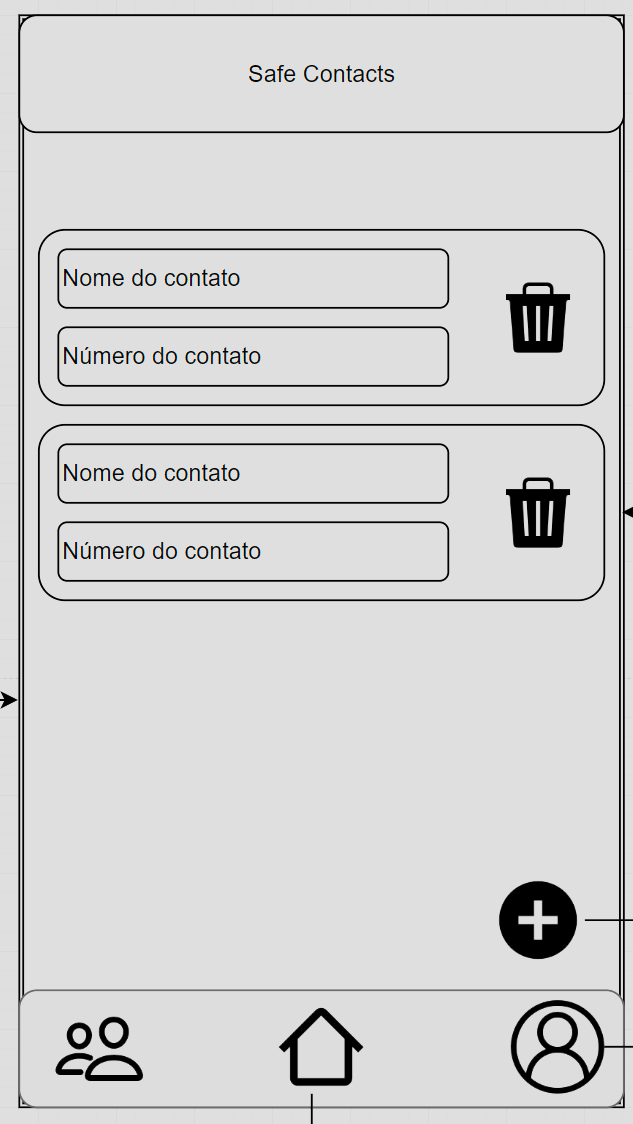
\includegraphics[width=0.2\linewidth]{images/wire-tela-listagem-contatos.png}\\
  \end{center}
  \caption[Wireframe Tela Listagem de contatos]{Wireframe Tela Listagem de contatos}
  \label{fig:wireframe-tela-listagem-contatos}
  \legend{Fonte: Próprio Autor}
\end{figure}
\pagebreak
Na tela de listagem de contatos será exibidos alista de contatos seguros queo usuário já cadastrou no aplicatiov. Caso não haja nenhum contato cadastrado será exibida uma mensagem informativa de que ainda não foram cadsatrados contatos. 

Há um float action buttoncom ícone de + que remete a ação de adicionar algo em qualquer aplicativo. A interação é através do clique no botão que levará para a tela de cadastro do novo contato.

Os contatos serão exibidos em forma de lsitagem na tela onde cada contato teerá seu próprio card exibido. Cada card exibirá o nome e o telefone do contato seguro cadastrado, desta forma o usuário conseguirá identificar sem equívoco cada um dos seus contatos. Haverá um menu de contexto o qual a ser clicado o usuário conseguirá acessar as funções de editar e deletar os conttos já cadastrados. Uma vez que o wireframa foi utilizado nesta análise, o menu de ocntexto será possível ser visualizado na imagem do prótotipo final. 

A tela seguirá o mesmo padrão das telas principais, mantendo a bottom bar no final da tela com os três ícones das funcionalidades principais indicando a navegação. 
\begin{comment}
	\begin{alineas}
		\item Tipo de interface e interação
		
		O tipo de interface utilização será de interface gráfica com listagem. A interação será feita através de gesto de rolagem na tela e com clique para ações. 
		\item Metáforas
		
		A BottomBar contém ícones os quais remetem as funcionalidades do aplicativo. O ícone com dois bonecos remete a uma lista de contatos. O ícone da casa remete a tela principal de qualquer aplicativo. Já o ícone circular com boneco dentro remete ao perfil em qualquer aplicação. 
		
		A própria BottomBar já remete a ideia de que é possível navegar entre essas três telas sem que tenha que sair deste menu em si.
		O ícone de lixeira será utilizado em cada card de contato indicando que ao clicar ali será executada a ação de deleção do contato seguro correspondente.
		
		\item Aprendizibilidade
		
		Previsibilidade – Ao clicar na lixeira de um determinado contato seguro o usuário receberá um alert em forma de Toast indicando que o contato seguro foi deletado.
		
		Capacidade de sintetização – Ao excluir um contato seguro com sucesso a tela de listagem de contatos é atualizada para retirar o contato seguro que foi removido.
		
		Familiaridade – Não se aplica.
		
		Consistência – Não se aplica. 
		
		Generalização – Não se aplica.
		
		\item Flexibilidade
		
		Iniciativa de diálogo – Não se aplica.
		
		Multitarefa – Não se aplica.
		
		Migração de atividade – Não se aplica.
		
		Substitutividade – Não se aplica.
		
		Personalização – Não se aplica.
		
		\item Robustez
		
		Observabilidade – Ao excluir um contato com sucesso o estado da tela de listagem é atualizado com a nova lista sem o contato que foi deletado.
		
		Recuperabilidade – O contato somente é deixado de ser exibido caso tenha ocorrido com sucesso a deleção. Em caso de insucesso é exibido um alerta em formato de Toast para o usuário indicando para que ele refaça a operação.
		
		Capacidade de resposta – Será exibido para o usuário um alerta em formato Toast indicando a deleção do contato seguro.
		
		Conformidade de realização de atividades – Não se aplica
	\end{alineas}
\end{comment}

\subsection{Tela 7 - Tela Pedidos de ajuda enviados}
\begin{figure}[h]
  \begin{center}
  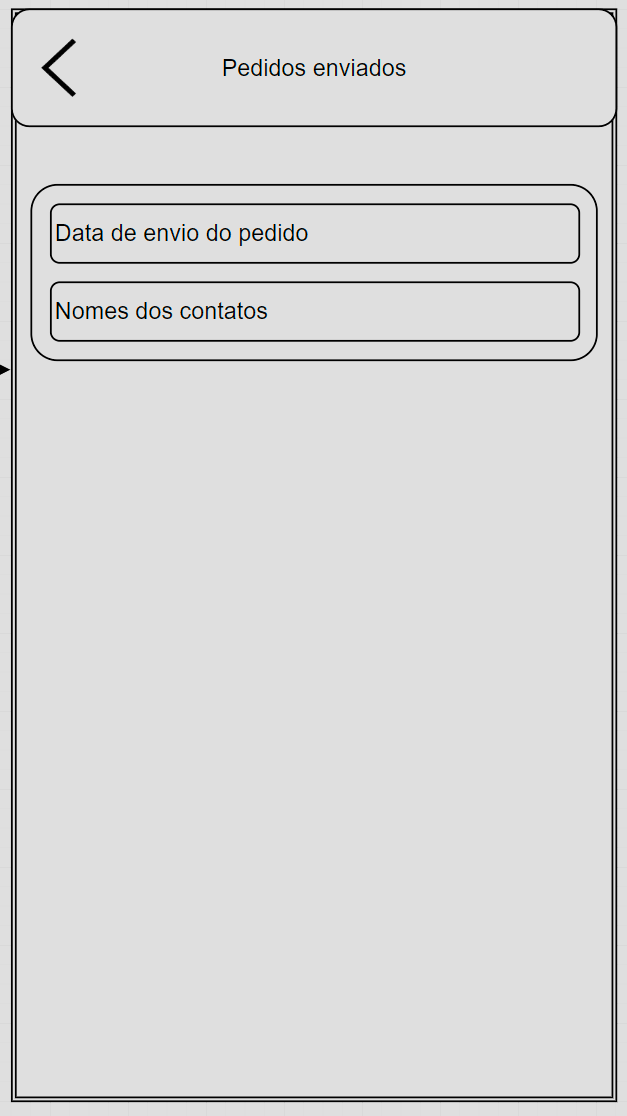
\includegraphics[width=0.2\linewidth]{images/wire-tela-pedidos-enviados.png}\\
  \end{center}
  \caption[Wireframe Tela Pedidos de ajuda enviados]{Wireframe Tela Pedidos de ajuda enviados}
  \label{fig:wireframe-tela-pedidos-ajuda}
  \legend{Fonte: Próprio Autor}
\end{figure}
\clearpage
\begin{comment}
\begin{alineas}
  \item Tipo de interface e interação
  
Será utilizada nessa tela o tipo de interface de listagem. A interação será através de scroll na tela. 
  \item Metáforas
  
Botão com ícone de seta para esquerda será exibido no canto superior esquerdo da AppBar indicando que irá retornar para tela anterior.
  \item Aprendizibilidade
  
Previsibilidade – Não se aplica.

Capacidade de sintetização – Não se aplica

Familiaridade – Não se aplica.

Consistência – Não se aplica.

Generalização – Não se aplica.
  \item Flexibilidade
  
Iniciativa de diálogo – Não se aplica.

Multitarefa – Não se aplica.

Migração de atividade – Não se aplica.

Substitutividade – Não se aplica.

Personalização – Não se aplica.

  \item Robustez
  
Observabilidade – Não se aplica.

Recuperabilidade – Ao obter erro na busca dos pedidos de socorro enviado do usuário, será emitido um alerta em forma de Toast indicando o erro e pedindo para que ele saia e entre novamente na tela de listagem. 

Capacidade de resposta – Indicar ao usuário quando não houver dados na listagem para serem exibidos.

Conformidade de realização de atividades – Não se aplica.

\end{alineas}
\end{comment}
Nesta tela serão exibidos os pedidos de socorro enviados em forma de listagem. Cada pedido será identificado em um card. Neste card conterá a data do pedido enviado e a localização de onde ele foi enviado. Será possível clicar no link das coordenadas de localização e ser direcionado para o aplicativo de mapas do usuário. O link será exibido com um sublinhado indicando que é um elemento clicavel como acontece em qualquer aplicativo.
\section{Avaliação de Usabilidade}
\subsection{Respostas das avaliações}
As respostas das avaliações dos usuários  e dos avaliadores especialistas podem ser encontradas no Anexo A deste documento.
\subsection{Correções e melhorias}
O protótipo se mostrou muito agradável aos participantes das avaliações. Alguns foram elencados e serão trabalhados para que sejam feitas as alterações. Alguns pontos foram bastante mencionados e são elencados abaixo.
\begin{itemize}
\item Alteração de contato – Será adicionado um botão ou menu de contexto com apresentará a opção de edição do contato já salvo para que não seja preciso excluir um contato primeiro para depois adicionar seu novo número.
\item Exclusão de contato – Será adicionada uma confirmação para prevenir de uma exclusão de contato acidental.
\item Configurações – Será alterado o título da tela de configurações para corresponder com a tela.
\item Ícone de logout – Será buscado um novo ícone ou repaginado o ícone atual para ficar mais intuitivo. 
\item Alteração de mensagem padrão – Será adicionado um feedback após realizar a alteração da mensagem para que fique mais claro de que a ação ocorreu com sucesso.
\item Campo de busca – Será adicionado um hint ao campo de busca informando o que o usuário deve preencher.
\item Botões de voltar – Diminuição dos ícones de voltar nas telas que possuem.
\end{itemize}
 
\subsection{Nova heurística}
Uma nova heurística a ser introduzida para interfaces mobile acredito que possa ser a opção de login com redes sociais. Hoje em dia é sim muito comum já termos essa opção nos aplicativos, porém ainda existem aqueles que não possuem essa funcionalidade. Essa heurística poderia avaliar a possibilidade de se colocar esse tipo de login, ou seja, se é viável ou se não se aplica dependendo do tipo de sistema.

\section{Conclusões sobre as avaliações}
Após recebidas e analisadas as avalições foi possível perceber que o protótipo se mostra muito promissor. Apesar de poucos apontamentos alguns deles se tornaram bastante perceptíveis visto que mais de um avaliador comentou sobre o mesmo problema. 

Pontos de acessibilidade a serem ajustados
\begin{itemize}
\item Alteração do nome da Tela 7 para condizer e identificar unicamente a tela de configurações
\item Criação de tooltip para cada menu de ação na tela 6 para assim melhor informar o que cada menu faz
\item Atentar ao uso do mapa na codificação para garantia de permissões necessárias.
\item Aplicar hint ao campo de busca para melhor definição do que se espera como entrada
\item Adicionar tolltip ao botão de adicionar contato seguro para melhor acessibilidade
\item Melhorar a formatação dos rótulos dos campos do formulário de cadastro de contato
\item Aplicação de visual de link na listagem de pedidos enviados na tela 8
\item Reavaliar o contraste dos botões dos dialogs
\end{itemize}



\chapter{Prototipação}

A prototipação de aplicativos móveis representa uma etapa fundamental no processo de desenvolvimento de software, constituindo-se como uma metodologia essencial para validação de conceitos, refinamento de funcionalidades e otimização da experiência do usuário antes da implementação final. Segundo estudos recentes, a experiência do usuário, interação usuário-produto e produtos digitais tornaram-se tópicos cada vez mais populares nas disciplinas de design nos últimos anos, evidenciando a crescente importância da prototipação no desenvolvimento de aplicações móveis \cite{sciencedirect_design_approaches}.

Definida como o processo de criação de versões preliminares e funcionais de uma aplicação, a prototipação permite aos desenvolvedores e designers testarem hipóteses, identificarem problemas de usabilidade e validarem soluções antes do investimento em desenvolvimento completo. A prototipação de aplicativos móveis é essencial para agilizar o desenvolvimento, melhorar a experiência do usuário e reduzir redesigns custosos \cite{decode_benefits}.

\section{Finalidades e Benefícios}

A prototipação de aplicativos móveis serve a múltiplos propósitos estratégicos no ciclo de desenvolvimento de software. Primeiramente, funciona como uma ferramenta de validação de conceitos, permitindo que equipes testem ideias e funcionalidades de forma iterativa e com baixo custo. Os protótipos de aplicativos móveis são poderosos e benéficos, oferecendo vantagens significativas em termos de economia de recursos e otimização de resultados \cite{gojilabs_essential}.

Entre os principais benefícios identificados na literatura, destaca-se a redução significativa de riscos de projeto. A prototipação oferece insights para refinar ainda mais a aplicação, sendo uma fase importante no desenvolvimento de aplicativos móveis \cite{softsuave_guide}. Adicionalmente, o processo facilita a comunicação entre stakeholders, permitindo visualização concreta de ideias abstratas e alinhamento de expectativas \cite{okoone_benefits}.

Atualmente, mais de 5,2 bilhões de dispositivos móveis únicos estão ativos mundialmente, destacando a escala massiva e o alcance da tecnologia móvel \cite{netguru_prototyping}. Este contexto reforça a importância estratégica da prototipação, considerando que dispositivos móveis representam 54\% de todo o tráfego web global, indicando uma mudança em direção a padrões de consumo mobile-first \cite{netguru_prototyping}.


\section{Aplicações Contemporâneas}

O campo da prototipação de aplicativos móveis tem evoluído significativamente com a incorporação de tecnologias emergentes. O mercado de aplicativos móveis é caracterizado por um grande número de aplicações frequentemente desenvolvidas por empresas menores, o que torna a prototipação ainda mais crucial para validação de viabilidade antes do investimento em desenvolvimento completo \cite{researchgate_ai_prototyping}.

Estudos recentes demonstram aplicações inovadoras da prototipação, incluindo o desenvolvimento de protótipos de aplicativos móveis focados na melhoria do aprendizado na área de matemática, utilizando metodologia Design Sprint para determinar características de usabilidade e aceitação por estudantes \cite{salud_ciencia_prototyping}. Estas aplicações evidenciam o potencial da prototipação não apenas como ferramenta de desenvolvimento, mas também como instrumento de pesquisa e inovação educacional.

\section{Considerações Metodológicas}

A implementação efetiva da prototipação requer consideração cuidadosa de aspectos metodológicos e ferramentais. Aprender a dominar a prototipação de aplicativos móveis pode economizar custos, melhorar a satisfação do usuário e agilizar o processo de desenvolvimento através de ferramentas efetivas \cite{decode_best_practices}.

A execução de protótipos pode fornecer insights para refinar ainda mais a aplicação, sendo fundamental seguir melhores práticas estabelecidas na literatura para maximizar os benefícios do processo \cite{ossisto_guide}. A seleção adequada de ferramentas e metodologias deve considerar fatores como complexidade do projeto, recursos disponíveis e objetivos específicos de validação.


\section{Protótipo SheSafe}

\subsection{Protótipo inicial}
\begin{figure}[h]
	\begin{center}
		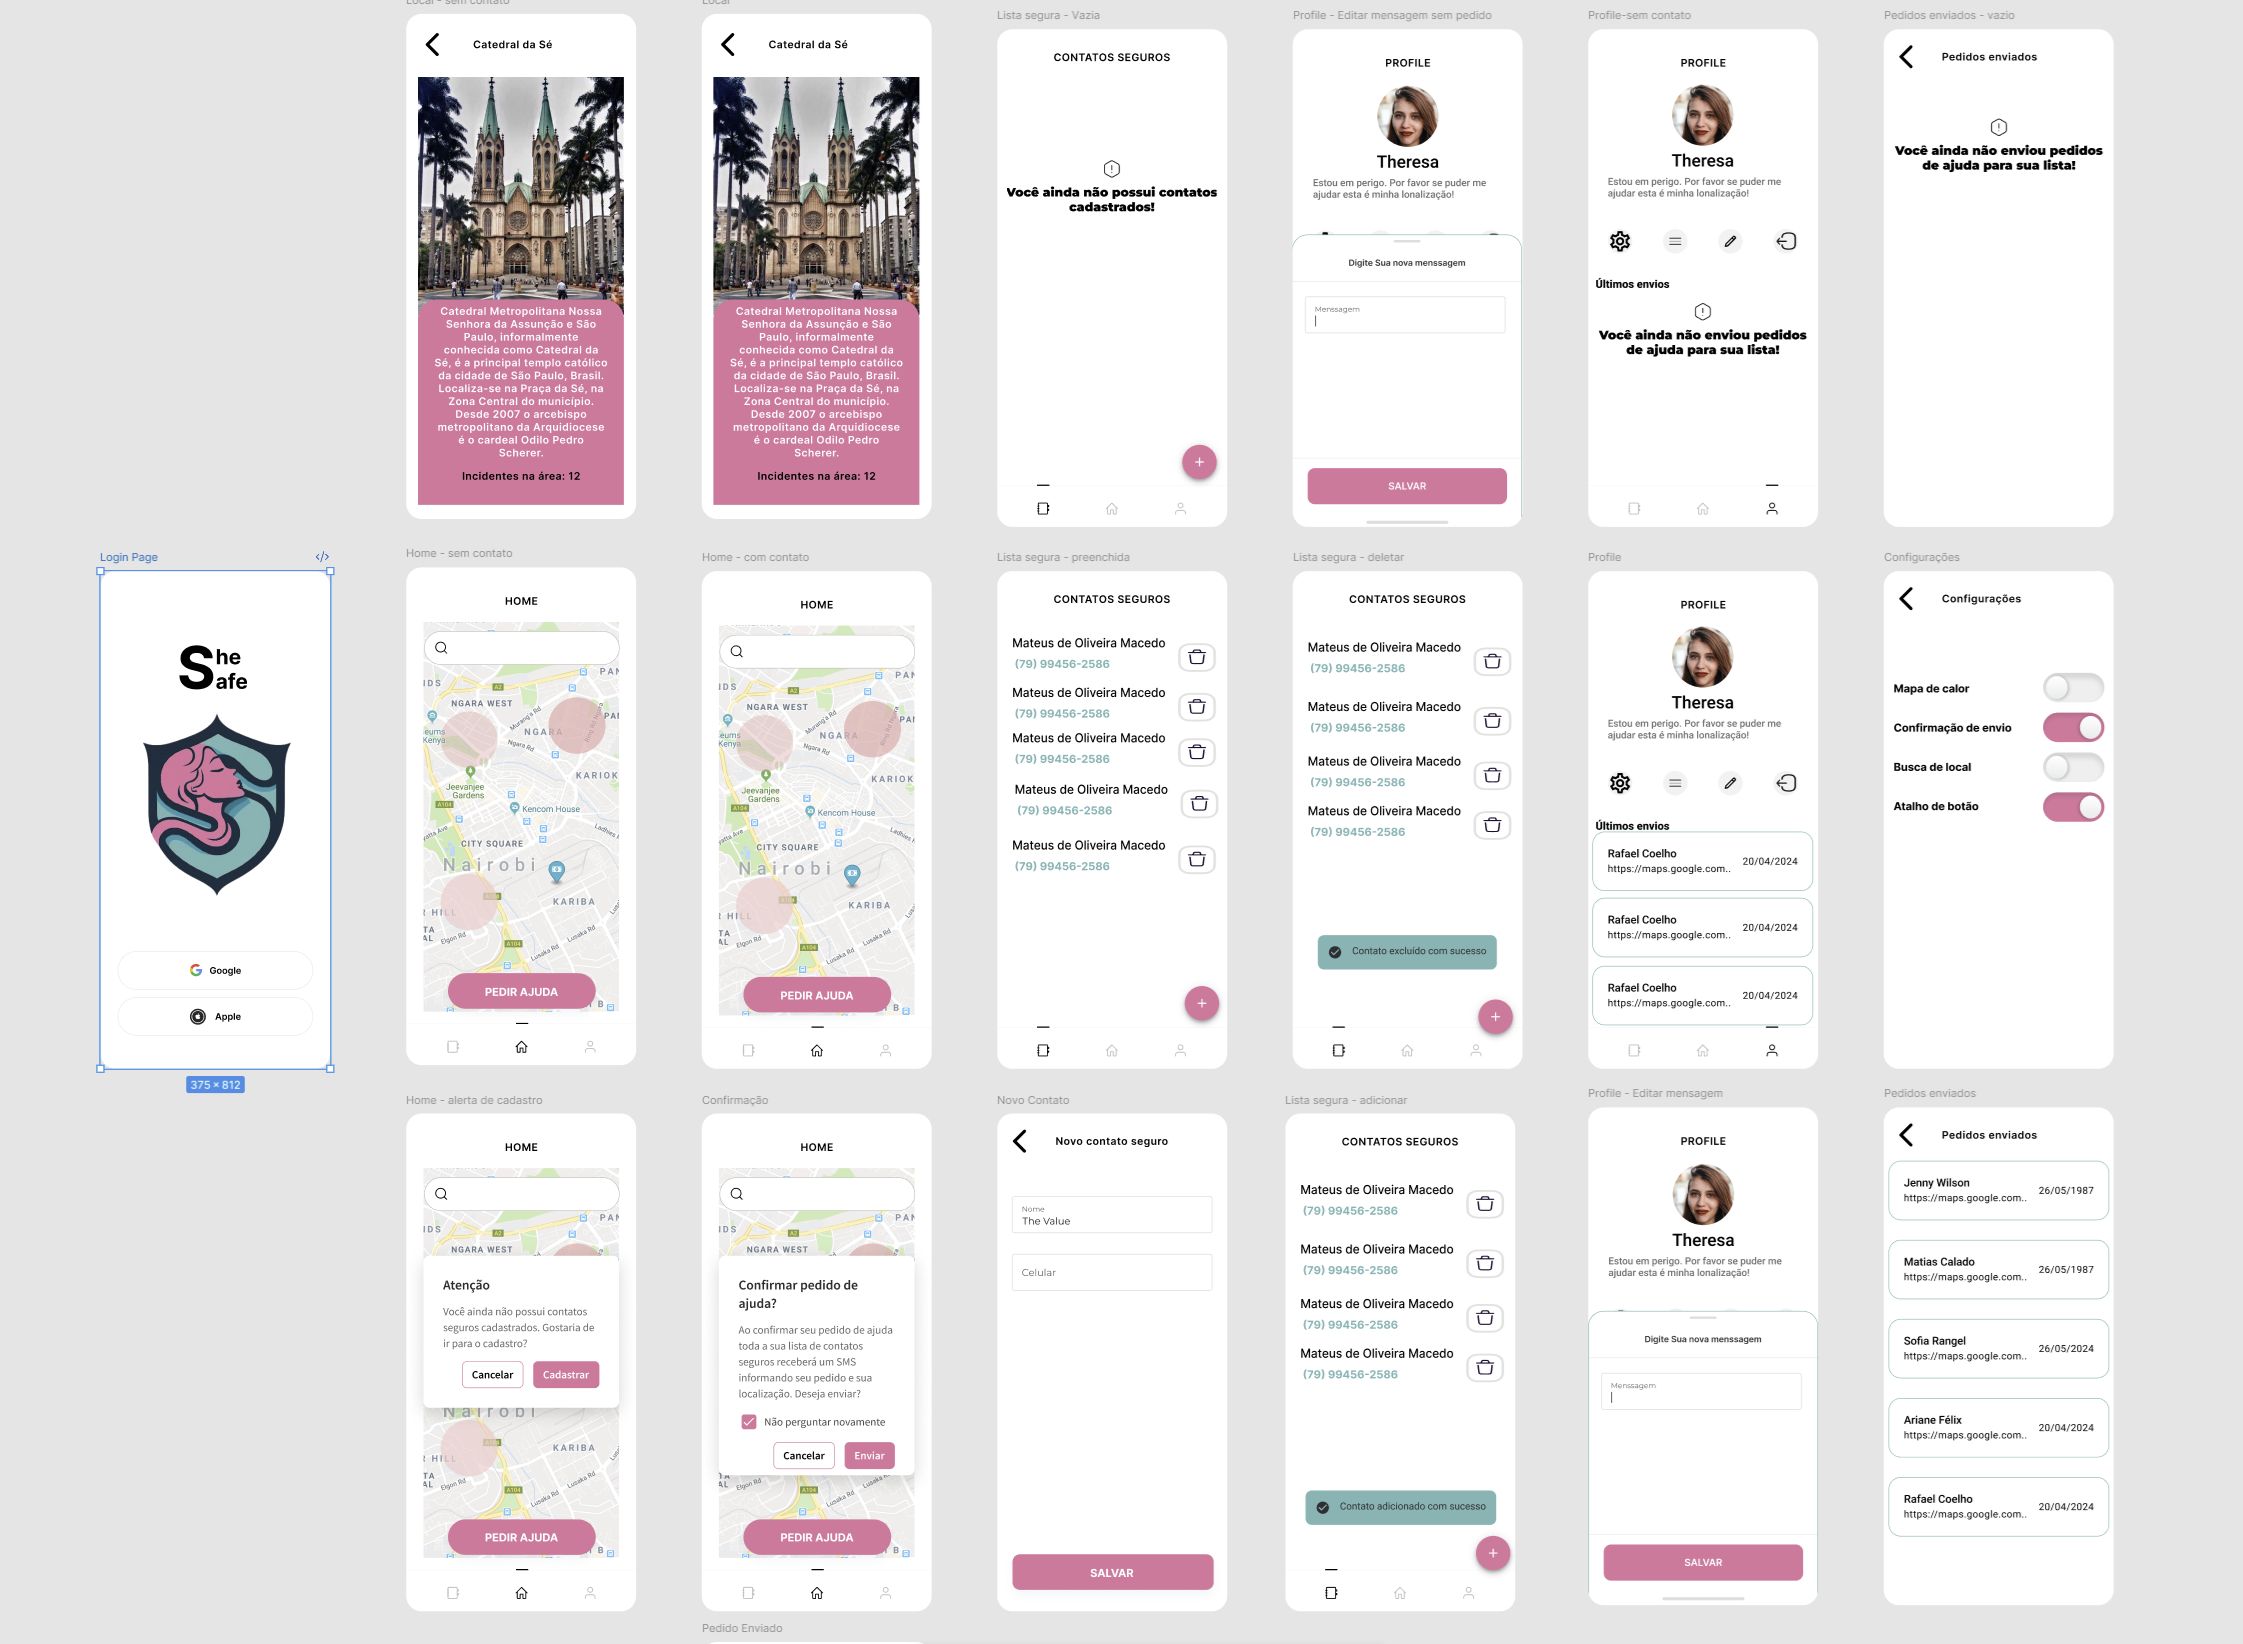
\includegraphics[width=0.8\linewidth]{images/prototipo-inicial.png}\\
	\end{center}
	\caption[Pr]{Protótipo inicial}
	\label{fig:prototipo-inicial}
	\legend{Fonte: Próprio Autor}
\end{figure}
\pagebreak

O protótipo inicial pode acessado através do link: \href{https://www.figma.com/proto/ZOxt5eHuQt0RjhagaDpuXU/SheSafe?type=design&node-id=26-369&viewport=1892%2C1064%2C0.71&t=gZiNpzVt2mGhuMDV-0&scaling=min-zoom&starting-point-node-id=26%3A653}{SheSafe - Protótipo Inicial}

\subsection{Protótipo final}
\begin{figure}[h]
	\begin{center}
		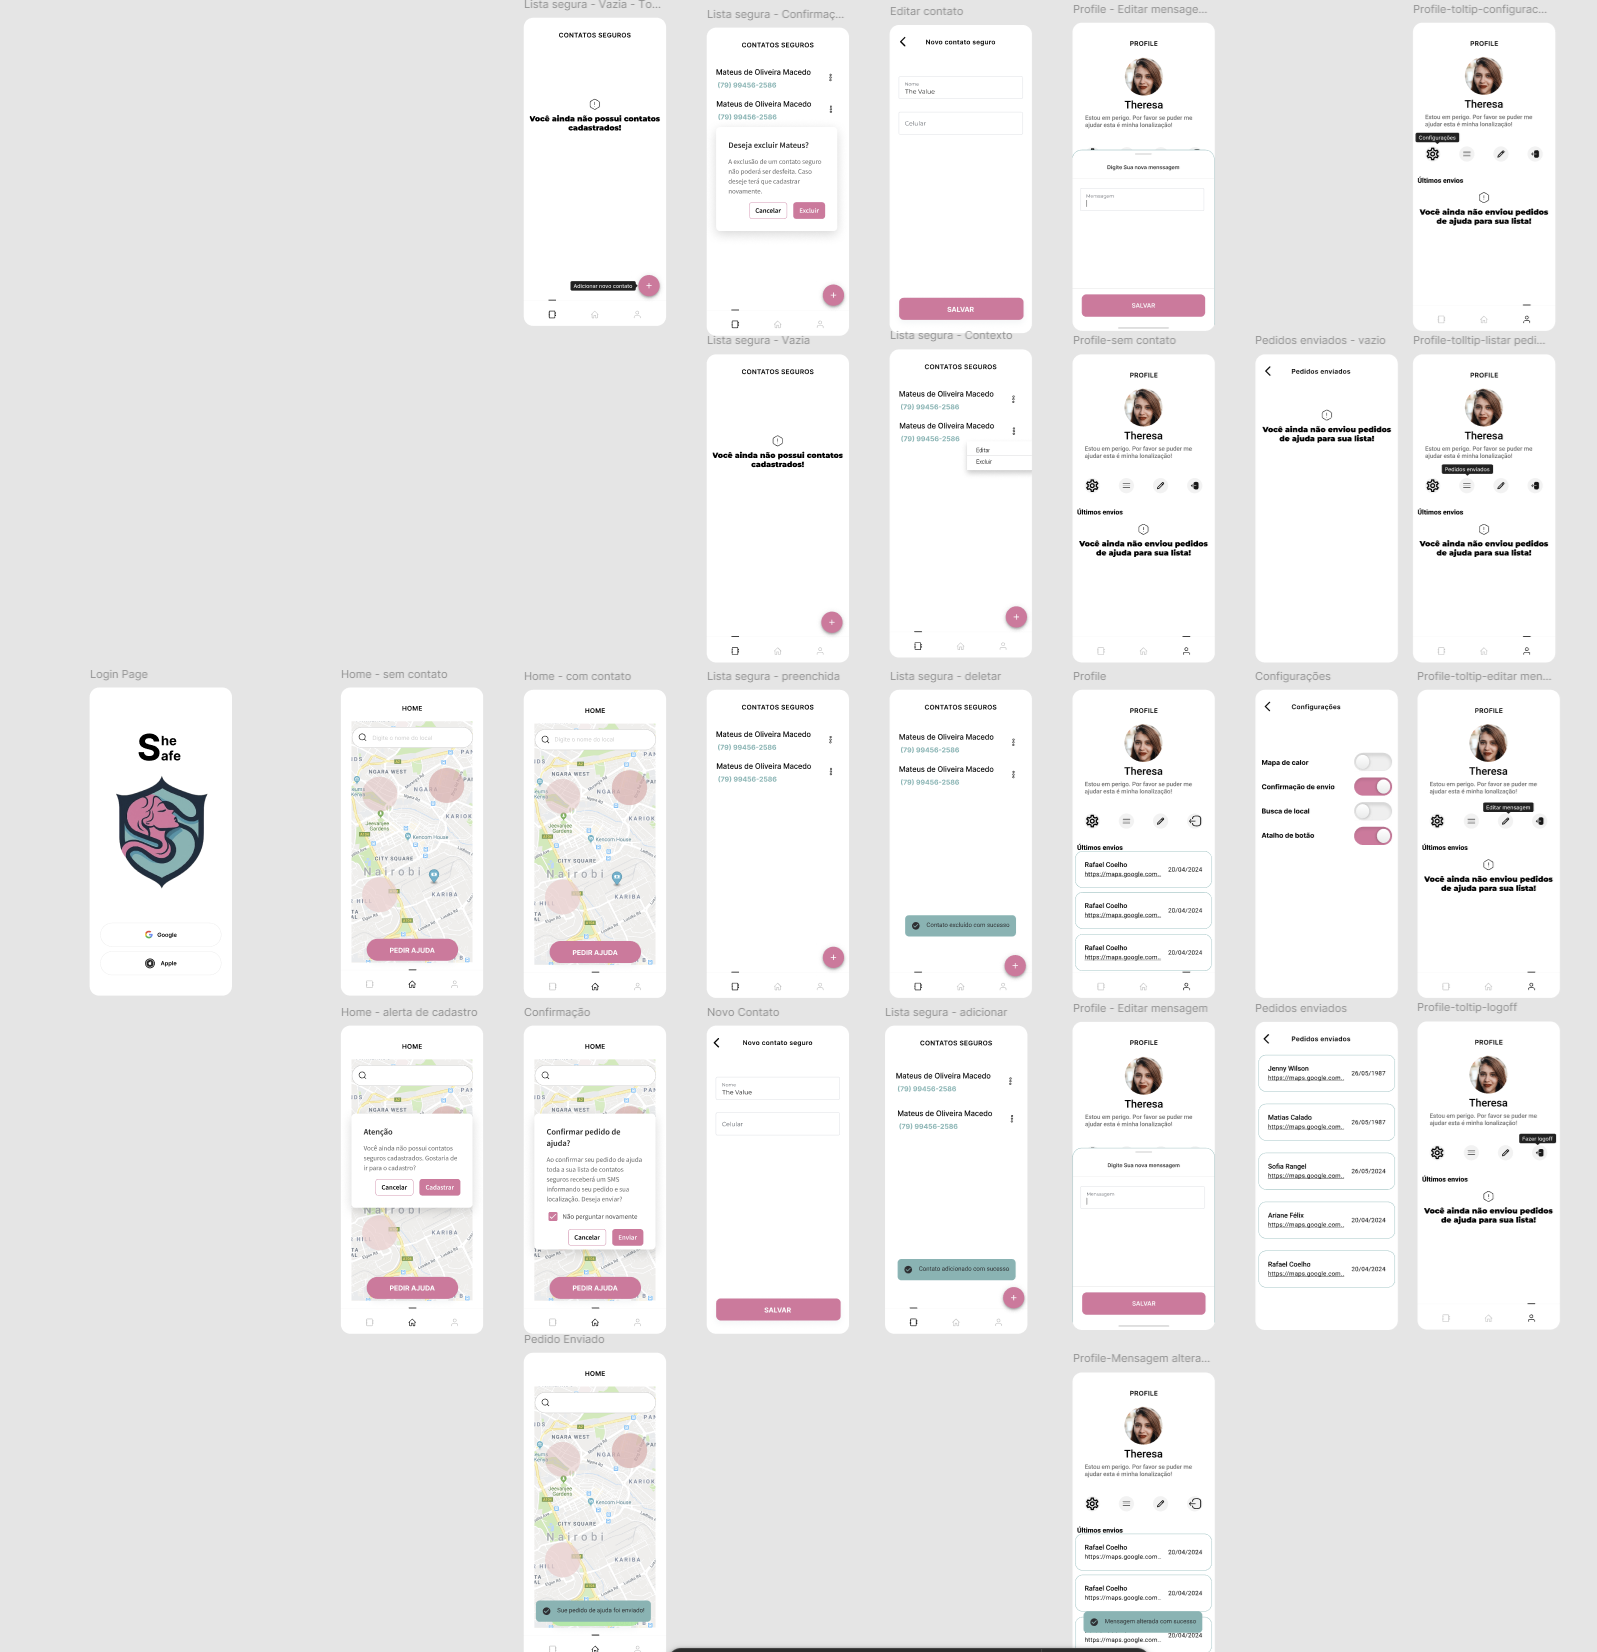
\includegraphics[width=0.7\linewidth]{images/prototipo-final.png}\\
	\end{center}
	\caption[Pr]{Protótipo final}
	\label{fig:prototipo-final}
	\legend{Fonte: Próprio Autor}
\end{figure}
\pagebreak
O protótipo final pode acessado através do link: \href{https://www.figma.com/proto/GALwTZKTsmvOVWX4JARmOB/SheSafe-Corrigido?node-id=26-653&viewport=2654%2C786%2C0.79&t=dkVCQTw83BbPw3KK-0&scaling=min-zoom&starting-point-node-id=26%3A653}{SheSafe - Protótipo Final}

Foi realizada uma cópia do projeto inicial para realizar as melhorias e alterações propostas pelas avaliações rasteira, heurística e de usabilidade.

\section{Melhorias Aplicadas}
Foram realizadas algumas mudanças no protótipo inicial até chegar no produto final. Tais melhorias foram realizadas com base nas avaliações aplicadas a público externo. Dentre elas estão:

\begin{itemize}
\item Tela 7 – alteração do título da tela para atender a corretamente ao que se propõe.
\item Tela de lista de contato – foi adicionado um menu de contexto com a opções de editar e excluir contato atendendo ao apontamento de não ser possível editar o contato.
\item Tela de listagem de contato – foi adicionado um dialog de confirmação de exclusão para atender ao apontamento de prevenção de exclusão acidental.
\item Tela 6 – foi alterado o ícone do menu de logoff para melhor exibir a intenção do menu.
\item Tela de alteração de mensagem – foi adicionada um feedback informando o sucesso da alteração da mensagem padrão do pedido de ajuda.
\item Campo de busca – adicionado hint explicativo para atender ao apontamento de não saber o que inserir no campo se busca.
\item Ícone de voltar – aplicada a redução do padrão de tamanho do ícone de voltar para atender ao apontamento recebido.
\item Botão de adicionar contato – foi introduzido um click longo para exibir um toltip explicando o que a ação do botão faz.
\item Menu de ações tela 6 – foi adicionado um toltip para ação de pressionar e segurar para os menus de ações da tela 6 atendendo ao apontamento de não saber exatamente o que cada menu faz. Com o toltip o menu passa a ter uma mensagem de contexto informado o que sua ação está encarregada.
\item Card de pedido enviado – aplicado estilo sublinhado no link do maps que contêm a localização do usuário atendendo ao apontamento sobre não reconhecer como link na tela o texto.
\item Dialogs – aplicado um pouco mais de peso no fundo dos botões de ação que ficam internos dentro dos dialogs para um melhor contraste.

\end{itemize}
% ----------------------------------------------------------
% ELEMENTOS PÓS-TEXTUAIS
% ----------------------------------------------------------
\postextual

% Referências bibliográficas

\bibliography{referencias}

% Caso sejam necessários apêndices ou anexos em seu documento
% Use os ambientes abaixo

%% Apêndices
%
%% Inicia os apêndices
%\begin{apendicesenv}
%
%% Imprime uma página indicando o início dos apêndices
%\partapendices
%
%\chapter{Primeiro Apêndice}
%
%\chapter{Segundo Apêndice}
%
%\end{apendicesenv}
%
%
%% ----------------------------------------------------------
%% Anexos
%% ----------------------------------------------------------
\begin{anexosenv}

% Imprime uma página indicando o início dos anexos
\partanexos

\chapter{Avaliações Heurística da Interface }

\includepdf[pages=-]{anexos/AnexoA.pdf}

%\chapter{Segundo Anexo}
%\lipsum[31]

\end{anexosenv}

\end{document}
